\documentclass[12pt, a4paper, oneside, british]{report}
\usepackage{epigraph}
\usepackage{setspace}
\usepackage{gensymb}
\usepackage[dvipsnames]{xcolor}
\usepackage[british]{babel}
\usepackage{amssymb}
\usepackage{amsmath}
\usepackage{pgfplotstable}
\usepackage{pgfplots}
\usepackage{natbib}
\usepackage[hyphens]{url}

%To Include PDFs
\usepackage{pdfpages}
\usepackage{longtable}

\bibliographystyle{abbrvnat}

\usepackage{colortbl}
\usepackage{adjustbox} 

\usepackage{textcomp}

%Diagramme
\usepackage{pgfplots}
\usepackage{pgfplotstable}

\usepackage[singlelinecheck=false,font={footnotesize, it}, tablewithin=section,
figurewithin=section,format=hang]{caption}

\usepackage{multirow}
\usepackage{footnote}
\makesavenoteenv{tabular}
%To Use Float Barrier
\usepackage{placeins}

%For Listings
\usepackage{listings}
\usepackage{lstlinebgrd}
% DOS-Fontstyle
\newenvironment{DOS_Font}{\footnotesize\color{black}\rmfamily}{\par}

\lstdefinestyle{DOS}
{
    backgroundcolor=\color{white},
    basicstyle=\footnotesize\color{black}\rmfamily,
    breaklines = true,
    breakatwhitespace=true,
    captionpos=rb
}

\lstdefinestyle{DOSScriptsize}
{
    backgroundcolor=\color{white},
    basicstyle=\footnotesize\color{black}\rmfamily,
    breaklines = true,
    breakatwhitespace=true,
    captionpos=rb
}

\lstdefinestyle{Wireshark}
{
    backgroundcolor=\color{white},
    basicstyle=\footnotesize\color{black}\rmfamily,
    captionpos=rb,
    breaklines=true,
    breakatwhitespace=true,
    tabsize=1,
    frame=single
}

\lstdefinestyle{WiresharkTiny}
{
    backgroundcolor=\color{white},
    basicstyle=\tiny\color{black}\rmfamily,
    captionpos=rb,
    breaklines=true,
    breakatwhitespace=true,
    tabsize=1,
    frame=single
}

\lstdefinestyle{WiresharkScriptSize}
{
    backgroundcolor=\color{white},
    basicstyle=\scriptsize\color{black}\rmfamily,
    captionpos=rb,
    breaklines=true,
    breakatwhitespace=true,
    tabsize=1,
    frame=single
}

%For Abbreviations
\usepackage[printonlyused]{acronym}

%For Headers and Footers
\usepackage{fancyhdr}
\renewcommand{\chaptermark}[1]{\markboth{#1}{}}
\renewcommand{\sectionmark}[1]{\markright{\arabic{section}.\ #1}}

\pagestyle{fancy}
\fancyhf{}
%\rhead{\itshape\nouppercase{\leftmark}} %shows chapter
\rhead{\itshape\nouppercase{\rightmark}}
\lfoot{Workshop \courseNumber - Acquistapace, Just, Lesnianski,
Schneider}
\rfoot{\thepage}
\renewcommand{\headrulewidth}{1pt}
\renewcommand{\footrulewidth}{1pt}

\newcommand{\prof}{Prof. Dr. rer. nat. Martin Zieher }
\newcommand{\courseNumber}{EE5503 }
\newcommand{\courseName}{Computer Networks }
\newcommand{\assignmentName}{TopicOfAssignment }
\newcommand{\assignmentAuthor}{Timo Acquistapace }
\newcommand{\studentNumber}{1644604 }
\begin{document}
\onehalfspacing
\setlength\epigraphrule{0pt}
\setlength{\epigraphwidth}{0.8\textwidth}
\renewcommand{\epigraphflush}{flushleft}

\bibliography{resources}
\begin{titlepage}
	\flushright
	
\includegraphics[width=0.50\textwidth]{res/Brunel_University_Logo.png}\par
	\centering
	\line(1,0){390}\\
	\vfill
	{\scshape\Large Master Course \\
	Distributed Computing Systems Engineering \par}
	\vspace{1.5cm}
	{\scshape\Large Workshop \courseNumber: \par}
	{\Huge\bfseries \assignmentName\par}
	\vspace{1.5cm}
	
	\begin{tabular}{rl}
	{\itshape \assignmentAuthorOne } & {\itshape \studentNumberOne }\\
	{\itshape \assignmentAuthorTwo } & {\itshape \studentNumberTwo }\\
	{\itshape \assignmentAuthorThree } & {\itshape \studentNumberThree
	}\\
	{\itshape \assignmentAuthorFour } & {\itshape \studentNumberFour
	}\\
	\end{tabular}
		
	\vspace{1cm}
	supervised by\par
	\prof

	\vfill
	\line(1,0){390}
	\flushleft
% Bottom of the page
	{\large \today\par}
\end{titlepage}
\pagenumbering{gobble}

\tableofcontents 
\newpage
% \begin{raggedleft}
% \begin{huge}
% \textbf{List of Abbreviations}
% \end{huge}
% \end{raggedleft}

\section*{List of Abbreviations}

\begin{acronym}[abcdefghijklmno]
 \input{contents/abbreviations.txt}
\end{acronym}
%\setcounter{chapter}{2}
\setcounter{page}{1}
\pagenumbering{arabic}

\chapter{Introducing TSMW}
\vspace{-1cm}
\epigraph{\textbf{Author: } Wojciech Lesnianski}

\vspace{-1cm}
\begin{table}
\renewcommand\arraystretch{1}
\begin{tabular}{p{0.23\textwidth}p{0.23\textwidth}p{0.23\textwidth}p{0.23\textwidth}}
\begin{center}Markus\end{center} & 
\begin{center}Simon\end{center} & 
\begin{center}Wojciech\end{center} & 
\begin{center}Timo\end{center}
\\
\vspace{-1.2cm}\begin{center}Just\end{center} & 
\vspace{-1.2cm}\begin{center}Schneider\end{center} & 
\vspace{-1.2cm}\begin{center}Lesnianski\end{center} & 
\vspace{-1.2cm}\begin{center}Acquistapace\end{center}
\\
\vspace{-1cm}\begin{center}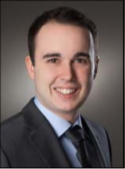
\includegraphics[width=0.2\textwidth]{res/intro/Markus.png}\end{center}
& 
\vspace{-1cm}\begin{center}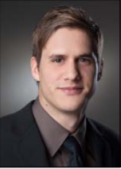
\includegraphics[width=0.2\textwidth]{res/intro/Simon.png}\end{center}
&
\vspace{-1cm}\begin{center}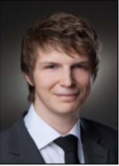
\includegraphics[width=0.2\textwidth]{res/intro/Ich.png}\end{center}
&
\vspace{-1cm}\begin{center}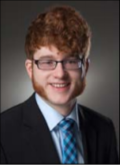
\includegraphics[width=0.2\textwidth]{res/intro/Timo.png}\end{center}
\\
\vspace{-1cm}\begin{center}Project Leader\end{center} & 
\vspace{-1cm}\begin{center}Dumbass\end{center} & 
\vspace{-1cm}\begin{center}Moron\end{center} &
\vspace{-1cm}\begin{center}Idiot \end{center}
\end{tabular}
\end{table}

\chapter{Aims, Objectives and expected Outcome}
\vspace{-1cm}
\epigraph{\textbf{Author: } Wojciech Lesnianski}

\vspace{-1cm}
In this chapter we will on the one hand discuss, what the overall aim of the
project is, and what the objectives are, which we want to achieve � either on
the way through the project or in its end. Furthermore we will forecast, what
our expected outcome of the project is and what the reasons for this forecast
are.

\section{Aim}
The aim of the project is to create a system which helps the user to bring out
his car from a parking position in the simplest, yet most convenient and
reliable way possible.

\section{Objectives}
The project's objectives are:

\begin{itemize}
  \item{Satisfaction of the customer \newline
	We measure our success rate with the satisfaction level of our customers.
	} 
	\item {Satisfaction of the end consumer \newline
	Since this is a system, our customer wants to make to provide support for his
	customers, his own satisfaction, and thus our success, will highly depend on
	this factor. We want to make his life easier, without asking too much of
	technical knowledge or making things so complicated to use, that he decides to
	do his actions without the help of our system. }
	\item{Creation of a satisfying hardware analysis \newline Since the system is
	supposed to use third party hardware for significant parts of the
	functionality, it is an objective to create a good analysis on the state of art
	of the needed variety of sensors.}
	\item {Create a System that is significant on the market \newline We want to
	create a system which other systems get compared to, when it comes to measuring
	the quality.}
\end{itemize}

\section{Expected Outcome}
The expected outcome of this project is, due to the lack of time and hardware:

\begin{itemize}
  \item A representative market analysis of current competition systems with the contrast to our product
  \item A representative market analysis on the needed hardware pieces for our
system 
  \item A solid and justified concept for a solution
  \item A proof of concept
\end{itemize}

\chapter{Requirement Analysis}
\vspace{-1cm}
\epigraph{\textbf{Author: } Markus Just, Wojciech Lesnianski}

\vspace{-1cm}
\section{Top-Level-Requirement}
The application should bring out a car from different parking positions
automatically.

\section{Functional Requirements}

\textbf{Required}

\begin{longtable}[l]{p{0.1\textwidth}p{0.8\textwidth}}
\textbf{3.2.1} & The application should be able to bring out the car from a parallel parking position\\
\textbf{3.2.2} & The application should be able to bring out the car from a perpendicular parking position\\
\textbf{3.2.3} & The application should be able to bring out the car from an angled parking position\\
\textbf{3.2.4} & The application should be able to work on the road side\\
\textbf{3.2.5} & The application should be able to work in a parking facility\\
\textbf{3.2.6} & The application should provide relevant sensor information to the driver in an graphical overview\\
\textbf{3.2.7} & The application should provide information about the current action to the driver in an aerial car view\\
\textbf{3.2.8} & It should always be possible for the driver to intervene the current process\\
\textbf{3.2.9} & The application should be able to work with right-hand traffic\\
\textbf{3.2.10} & The application should be able to work with left-hand traffic\\
\textbf{3.2.11} & The application should consider the traffic rules and should act properly\\
\textbf{3.2.12} & The application should bring the car out of the parking system in a way that after that process it is possible to enter it from all sides\\
\end{longtable}

\begin{raggedleft}
\textbf{Nice-to-have}
\end{raggedleft}

\begin{longtable}[l]{p{0.1\textwidth}p{0.8\textwidth}}
\textbf{3.2.13} & The application should work independent of the current weather conditions\\
\textbf{3.2.14} & The cars should have customizable skins, selectable by the user\\
\textbf{3.2.15} & The application should be remote-controllable by a mobile application if the user is within a defined range to the vehicle\\
\end{longtable}

\section{Non-functional Requirements}

\begin{longtable}[l]{p{0.1\textwidth}p{0.8\textwidth}}
\textbf{3.3.1} & The application must comply national safety regulations\\
\textbf{3.3.2} & The application should have a suitable design\\
\textbf{3.3.3} & The application should be integrated in the given car's entertainment system\\
\textbf{3.3.4} & The application's GUI should be easy to grasp for the user\\
\textbf{3.3.5} & The application should be easy to extend\\
\textbf{3.3.6} & The application should be secured against any kind of attack\\
\textbf{3.3.7} & The application should be integrateable in different sorts of vehicles\\
\textbf{3.3.8} & The application should be developed with C\#/.NET\\
\textbf{3.3.9} & The application�s GUI should be developed with WPF.\\
\end{longtable}

\chapter{Specification}
\vspace{-1cm}
\epigraph{\textbf{Author: } Wojciech Lesnianski}

\vspace{-1cm}
The following chapter describes the specification of the developed system. It is
based on the customer requirements and correspondence with the customer. This
chapter will be adjusted if requirements change, to provide clearance during the
development process, as well as the maintenance process after releasing the
system.

\section{Project Scope}
The system shall support a driver with taking his car out of a parking lot. The
system is designed to work with the cars of the customer. It should use sensors,
build around the car, to take the car out of every parking position in the most
convenient and safe way. The system should provide a graphical user interface
within the car display, to provide overview over the process of taking out the
car.

\section{Supported Parking Positions}
The two main parking positions shall be supported, as shown in the pictures
below:

\begin{figure}[h!]
  \centering
     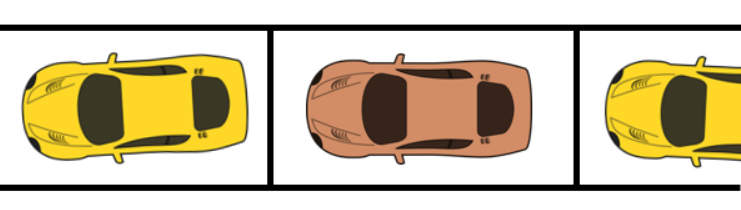
\includegraphics[width=\textwidth]
     {res/spec/Hintereinander.PNG}
     \captionsetup{justification=centering}
  \caption{Parallel Parking}
  \label{fig:project plan}
\end{figure}

\begin{figure}[h!]
  \centering
     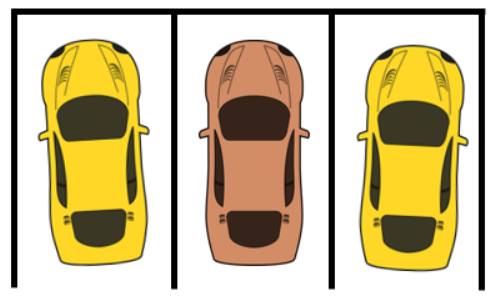
\includegraphics[width=\textwidth]
     {res/spec/Nebeneinander.PNG}
     \captionsetup{justification=centering}
  \caption{Perpendicular Parking}
  \label{fig:project plan}
\end{figure}

\FloatBarrier

A car moved out of a lengthwise parking lot has to face the same direction as
before being taken out, while a car taken out of a transversal parking lot is
moved $90^\circ$ clockwise when being taken out. Angled parking lots are
treated the same way as transversal parking lots, only the orientation of the car is not
changed by the whole $90^\circ$, but by a smaller amount. In all cases, the
cars have to leave the parking lot entirely, and must not enter the opposite lane at any
time of the process.

\section{Sensors}

The system uses a number of sensors placed on and within the automobile. They
are used to ensure a secure process of taking out the vehicle off the parking lot:

\begin{itemize}
 \item	Speed Sensor \newline 
Acquire the current speed 
 \item Distance Sensor \newline
Acquire the distances between the vehicle and obstacles
\end{itemize}

\section{Required Controls}

The parking system requires the control or a possibility to interact with a
number of car components to work properly and to its full potential:

\begin{itemize}
  
\item Transmission control \newline
Switch between forwards and reverse driving
\item Engine control \newline
Set the desired car velocity
\item Board computer control \newline
Display the user interface 
\item Brake control \newline
Decrease the velocity
\item Steering control \newline
Change the vehicles direction
\end{itemize}

The board computer is not mandatory for the system to work, but highly
recommended.

\section{Obstacles}
The parking assistance system shall be able to take obstacles into account.
There are two kinds of obstacles we are facing when running the process of
taking out a car of a parking lot:

\textbf{Static obstacles} \newline
Static obstacles are not moving themselves. Their distance towards our vehicle
controlled by the parking assistant system only changes by the movement of the
vehicle itself. We do not have to predict where the obstacle might be positioned
at some other point in time. Static obstacles are objects like:

\begin{itemize}
\item Parked cars
\item Houses 
\item Walls
\item Burgundy
\item Trees  
\end{itemize}

\textbf{Dynamic obstacles} \newline
Dynamic obstacles have a movement, or the potential to move during our process
of taking out the car of a parking lot. Their distance to our vehicle can change
without our car having any velocity. If there is any possibility, an obstacle
might interfere with our vehicle, or the predicted path of our vehicle, it has
to be taken into account during the process. If the distance between an obstacle
and our vehicle is reducing by a higher ration than the velocity of the car, the
car has to stop. Dynamic obstacles are objects like:

\begin{itemize}
\item Moving cars
\item Human beings
\item Animals  
\end{itemize}

\section{Country Regulations}

The system should primary work in Great Britain � thus the traffic rules of
Britain should be considered when running a process of taking the vehicle out of
the parking lot. The rules for the process do not differ in any country of
Europe by any other factor than the side of the road the cars are driving on.
Therefor there must be a setting to switch between:

\begin{itemize}
 \item Right-hand traffic
 \item Left-hand traffic (default)  
\end{itemize}

\section{Graphical User Interface}

The graphical user interface is a non-mandatory, but highly recommended part of
the system. It shall initiate the process of taking a car out of its parking
position. It shall be intuitive and use the corporate design of the customer.
Furthermore, it shall monitor the process by displaying the following
information to the driver:

\begin{itemize}
 \item	A top-down view of the car and the closest surroundings
 \item Predicted car route
 \item Vehicle velocity
 \item Driving direction
 \item Distance to the closest obstacles on each side of the car
 \item Warnings in case of dangerous situations  
\end{itemize}

\section{Implementation}

The system should be implemented with the programming language C#. For the
graphical user interface the framework WPF is to be used, as well as the
corporate design of the customer for WPC controls styling. For sensor
communication we will use CAN buses and extract the required information from
the streams. An SQL database will be supplied to assure fast processing of the
high amount of data in a small time and to ensure performance we will work with
stored procedures.

\chapter{Project Plan}
\vspace{-1cm}
\epigraph{\textbf{Author: } Markus Just}

\vspace{-1cm}
On the start of a project there are several things which have to be defined for
the organisation of the working process. Based on the specification which is
approved and signed by the client the initial planning is a crucial step to
achieve a successful project outcome. 

There are some major aspects which have to be considered when planning a
project:

\begin{itemize}
\item time which is needed to fulfill the accruing tasks
\item resources which are responsible to fulfil tasks
\item costs which emerge through the use of resources over a specific time
\end{itemize}

Planning these aspects is the initial step during the project. The period of
time is about 5 months while every team member's work hours are determined with
about 100 hours.

\section{Planning Aims}

The planning of the project doesn't only exist to have documentation about what
to be done. A good planning provides the possibility to measure the impacts on
the time/cost of different occurring scenarios during the project. The SMART
rule defines how project objectives should be defined:

\begin{itemize}
\item \textbf{S}pecific: goals should be defined clearly
\item \textbf{M}easurable: progress should be measurable
\item \textbf{A}ttainable: goals should meet specific targets 
\item \textbf{R}easonable: the goal should be achievable and realistic
\item \textbf{T}ime-bound: the goal should be bound to a fixed date 
\end{itemize}

In the next step, which is the definition of tasks, these rules have to be
considered. 

\section{Task Overview}
The initial step after defining the specification is to create and schedule the
tasks and milestones to achieve the fulfilling of the requirements. The aim is
to generate an overview over the things which have to be done and when they have
to be done. So each task gets a meaningful description, an estimated duration
and a starting date. To achieve this overview, the freeware tool GanttProject
has been used.

Normally not every task which has to be done can be defined beforehand, because
sometimes the customer requirements change during the development or it wasn't
possible to discover all necessary tasks on project start.

Because of the fact that the time period for this project is 5 months, while the
work hours of each team member is determined with about 100 hours, it was
decided that the initial planning starts in December while the actual
development of the system starts in March so that between these months the team
members are able to concentrate on working at their company and on other master
courses.

\begin{figure}[h!]
  \centering
     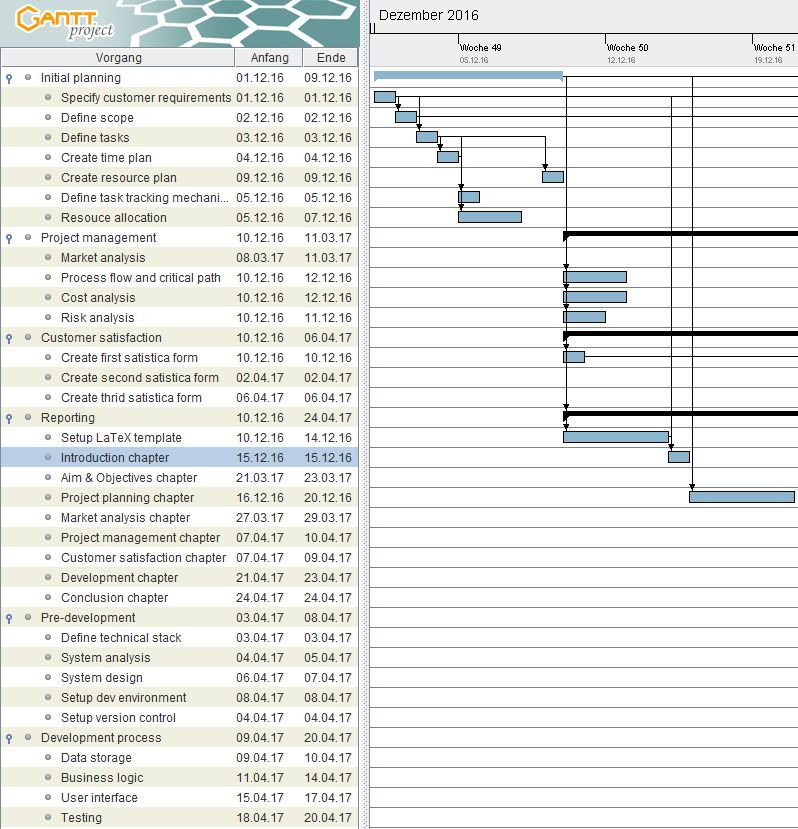
\includegraphics[width=1\textwidth]
     {res/projectPlan/timePlan1.JPG}
     \captionsetup{justification=centering}
  \caption{Final Project Plan}
  \label{fig:project plan}
\end{figure}

Figure \ref{fig:project plan} shows the layout of the GanttProject application
as well as the defined tasks for December 2016 in the chart. It also shows the
aspect that the tasks aren't independent from each other, e.g. the tasks can
only be created if the scope of the project is defined.

\section{Resource Overview}

As soon as the tasks are defined it is necessary to plan the human resources.
The module description states that each team member participates with 100 hours
of work in this project, so the tasks must be distributed consistent. It's the
aim that each team member works on the tasks which are related to their role,
however this can't be achieved 100\% accurately, so it may be the case that the
software architect works on a project management related task.

Because the time period of the project is almost 5 months, the initial planning
tasks are executed in December, while the real project work begins end of
February. This was coordinated with the acceptance of all team members.

The resource overview was also created with the freeware tool GanttProject and
looks as follows:  

\begin{figure}[h!]
  \centering
     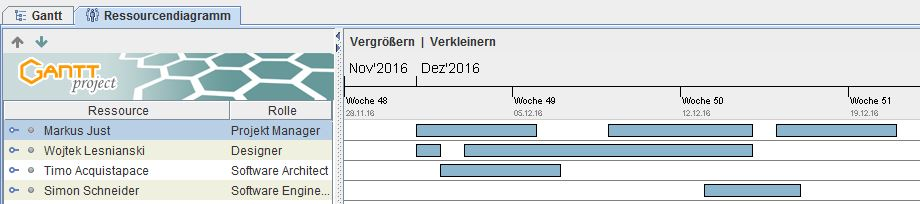
\includegraphics[width=1\textwidth]
     {res/projectPlan/ResourcePlan1.JPG}
     \captionsetup{justification=centering}
  \caption{Resouce Plan December}
  \label{fig:resource plan december}
\end{figure}

\begin{figure}[h!]
  \centering
     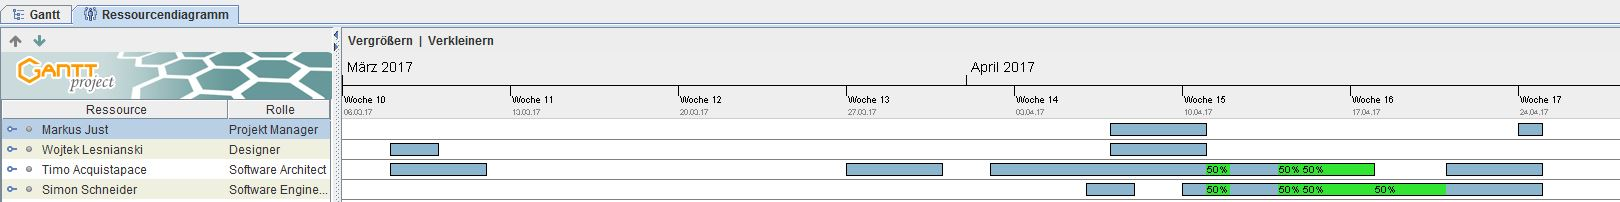
\includegraphics[width=1\textwidth]
     {res/projectPlan/ResourcePlan2.JPG}
     \captionsetup{justification=centering}
  \caption{Resource Plan March / April}
  \label{fig:resource plan march}
\end{figure}

\section{Cost Overview}

After the resource planning is done, it is now possible to look at the costs of
the different work phases as well as the total cost for the resources. Each team
member got a salary of 117\pounds/hour, so the resource cost of the whole
project can be initially calculated with 46.800\pounds (about 100 work hours for
each team member).

The GanttProject tool calculates the costs for each base task and its sub tasks,
which results in the following output that can be seen in table \ref{tab:cost
overview}.

\begin{table}[h!]
  \centering
\begin{adjustbox}{max width=\textwidth}
\begin{tabular}{|c|c|}
Task&Cost\\
\hline
\rowcolor{lightgray}Initial Planning&8.611\pounds\\
Project Management&9.360\pounds\\
\rowcolor{lightgray}Customer Satisfaction&2.246\pounds\\
Pre-Development&5.242\pounds\\
\rowcolor{lightgray}Development Process&7.114\pounds\\
Reporting&15.023\pounds\\
\rowcolor{lightgray}Total&47.596\pounds\\
\hline
\end{tabular}
\end{adjustbox}
\captionsetup{justification=centering}
  \caption{Cost Overview}
  \label{tab:cost overview}
\end{table}

These overview shows that the estimated costs for executing the defined tasks is
a bit higher than expected, but the difference is not seriously high, so it
isn't much of a problem.

\section{Task Tracking Mechanism}

GanttProject doesn't only provide mechanisms for project planning, it also
provides the possibility to track the current process. This can be achieved by
setting the initial plan as the base plan and after that, the real time spent on
a task can be entered. The GanttProject tool shows the impact on the whole time
plan when a task is finished late/early as it can be seen in figure
\ref{fig:project plan with finished tasks}:

\begin{figure}
  \centering
     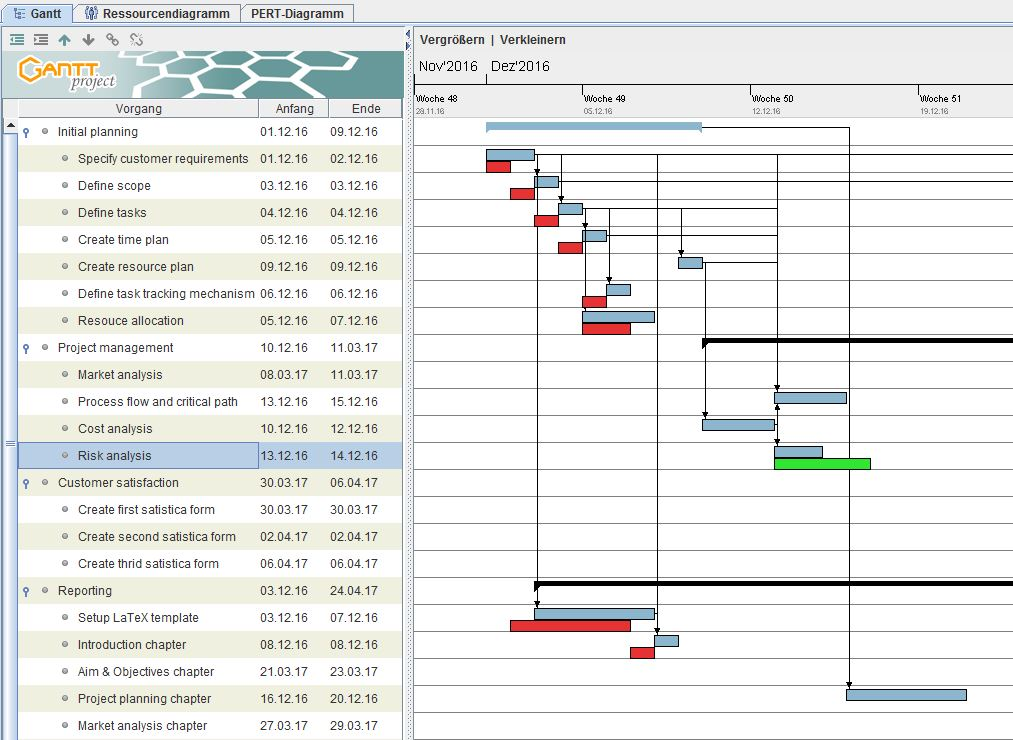
\includegraphics[width=1\textwidth]
     {res/projectPlan/Tracking.JPG}
     \captionsetup{justification=centering}
  \caption{Final Project Plan with Finished Tasks}
  \label{fig:project plan with finished tasks}
\end{figure}

The grey bars show the actual progress of the project. The red/green bars show
the differences to the initial plan. If the bar is red it means the initial
estimated time plan for this task couldn't be followed for this task. If the bar
is green it means this task has been finished earlier than expected.

Each team member should enter the beginning and the duration of the tasks he
finished to make sure that the progression of the project goes forward as it was
planned and the project can be successfully finished until the deadline.

\FloatBarrier

\section{Critical Path}

The ``critical path'' is a planning instrument, which has its origins in the
network plan technology. With its help it is possible to analyse impacts on the
time plan of a project if delays occur during a task execution. The critical
path is the succession of tasks which are interdependent and it indicates the
shortest time needed to finish a project. If one of the tasks belonging to the
critical path is delayed because of some circumstance, the whole project
execution time is delayed as well.

The critical path is useful to analyse which tasks are important and it gives
the possibility to prevent a large delay in finishing the project by
redistribute the resources or move other tasks, which are not part of the
critical path, to the end of the project without further impact on the project
duration.

To visualise the critical path, it is necessary to define the starting dates,
the duration and the dependencies between the tasks. After that each task is
visualised as a process bar and is connected via arrows to other depending
tasks. GanttProject provides the possibility to create a PERT-diagram, which
shows a graphic illustration of a project as a network diagram. Unfortunately
GanttProject isn't able to create a clear PERT-chart which can be pasted here,
so the complete diagram can be found in the appendix \ref{sec:pert}:

\begin{figure}
  \centering
     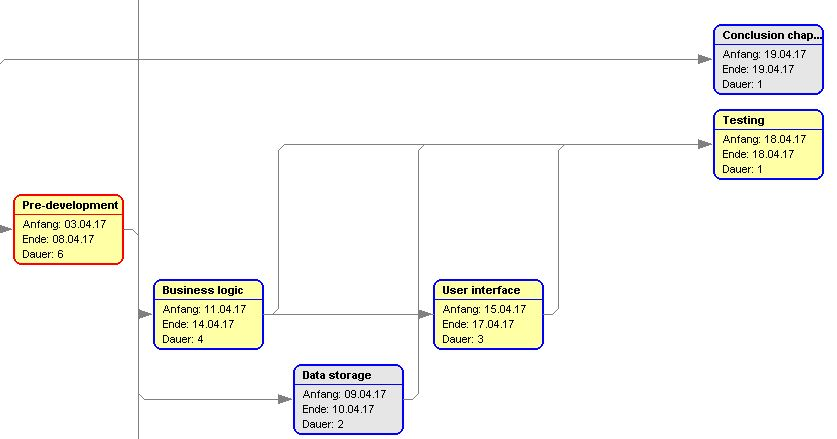
\includegraphics[width=1\textwidth]
     {res/projectPlan/criticalPathExtract4.JPG}
     \captionsetup{justification=centering}
  \caption{PERT-Diagram Extract}
  \label{fig:extract}
\end{figure}

\chapter{Resource Allocation}
\vspace{-0.85cm}
\epigraph{\textbf{Author: } Wojciech Lesnianski}

\vspace{-1cm}
Available resources were always one of the biggest goods Project
Managers had to work with, to keep customers happy. Especially with the growing agile approach
popularity, where development iterations become smaller, it is of high
importance to use all resources the most efficient way. Efficiency in this case,
does not always mean, to put the most fitting developer on a task, but also
consider where the other resources are allocated at the time. Putting a
developer on a task that is not fitting him perfectly might still be a good idea
if another developer would not be able to do anything otherwise.

\section{Methodology of Resource Allocation}
There are various methods which aim at the best possible resource allocation and
they all first require the user, possibly the project manager, to break down
jobs in tasks and classify the tasks and the resources in a specific way. The
better the breakdown and the classification is, the better the project manager
can allocate his resources.

For this project we will use the method described in the lectures of Dr. Ali
Mousavi (see \cite{ResAlloc}). 

This method focuses on classifying tasks and
identifying the best possible human resource to fulfill the task. First the
human resources get their Indicators of Capability:

\begin{itemize}
\item The Enablers (E) � cognitive capabilities, skills and roles
\item The Preferences (P) � personal traits
\item Past Attainments (A) � past experience in similar roles 
\end{itemize}

It takes an experienced project manager and good self-assessment of the
developer to put together a representative and well-founded list of enabler
properties.

In the following, we will calculate the impact and utilization of a specific
human resource on a specific job as an example. Since we are a small company we
take the job implementation as one big job which we separate into tasks (see
figure \ref{fig:table1}). After writing down the most important skills needed 
for the single tasks, we can
put them all together in a separate table, considering the highest $X$ (see
figure \ref{fig:table2}).

\begin{figure}
\centering
\captionsetup{justification=centering}
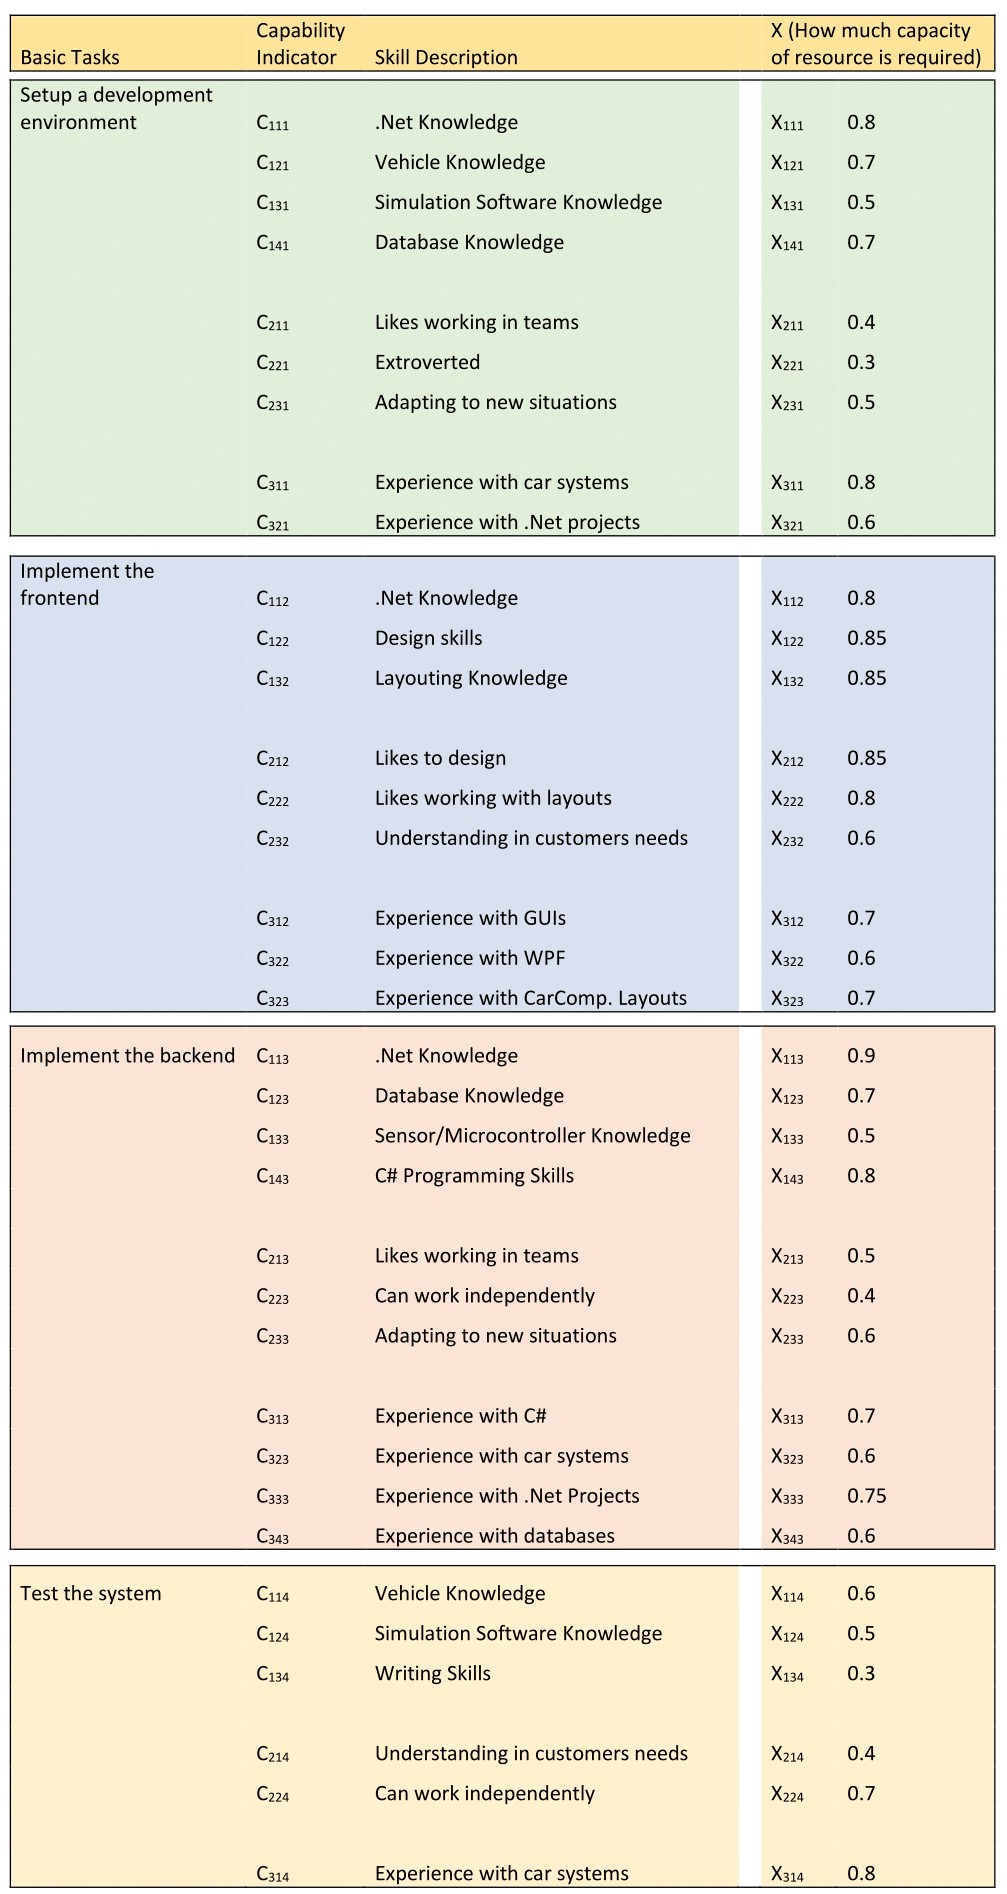
\includegraphics[width=0.75\textwidth]{res/resAlloc/Table1.jpg}
\caption{Task-Resource Matching}
\label{fig:table1}
\end{figure}

\begin{figure}
\centering
\captionsetup{justification=centering}
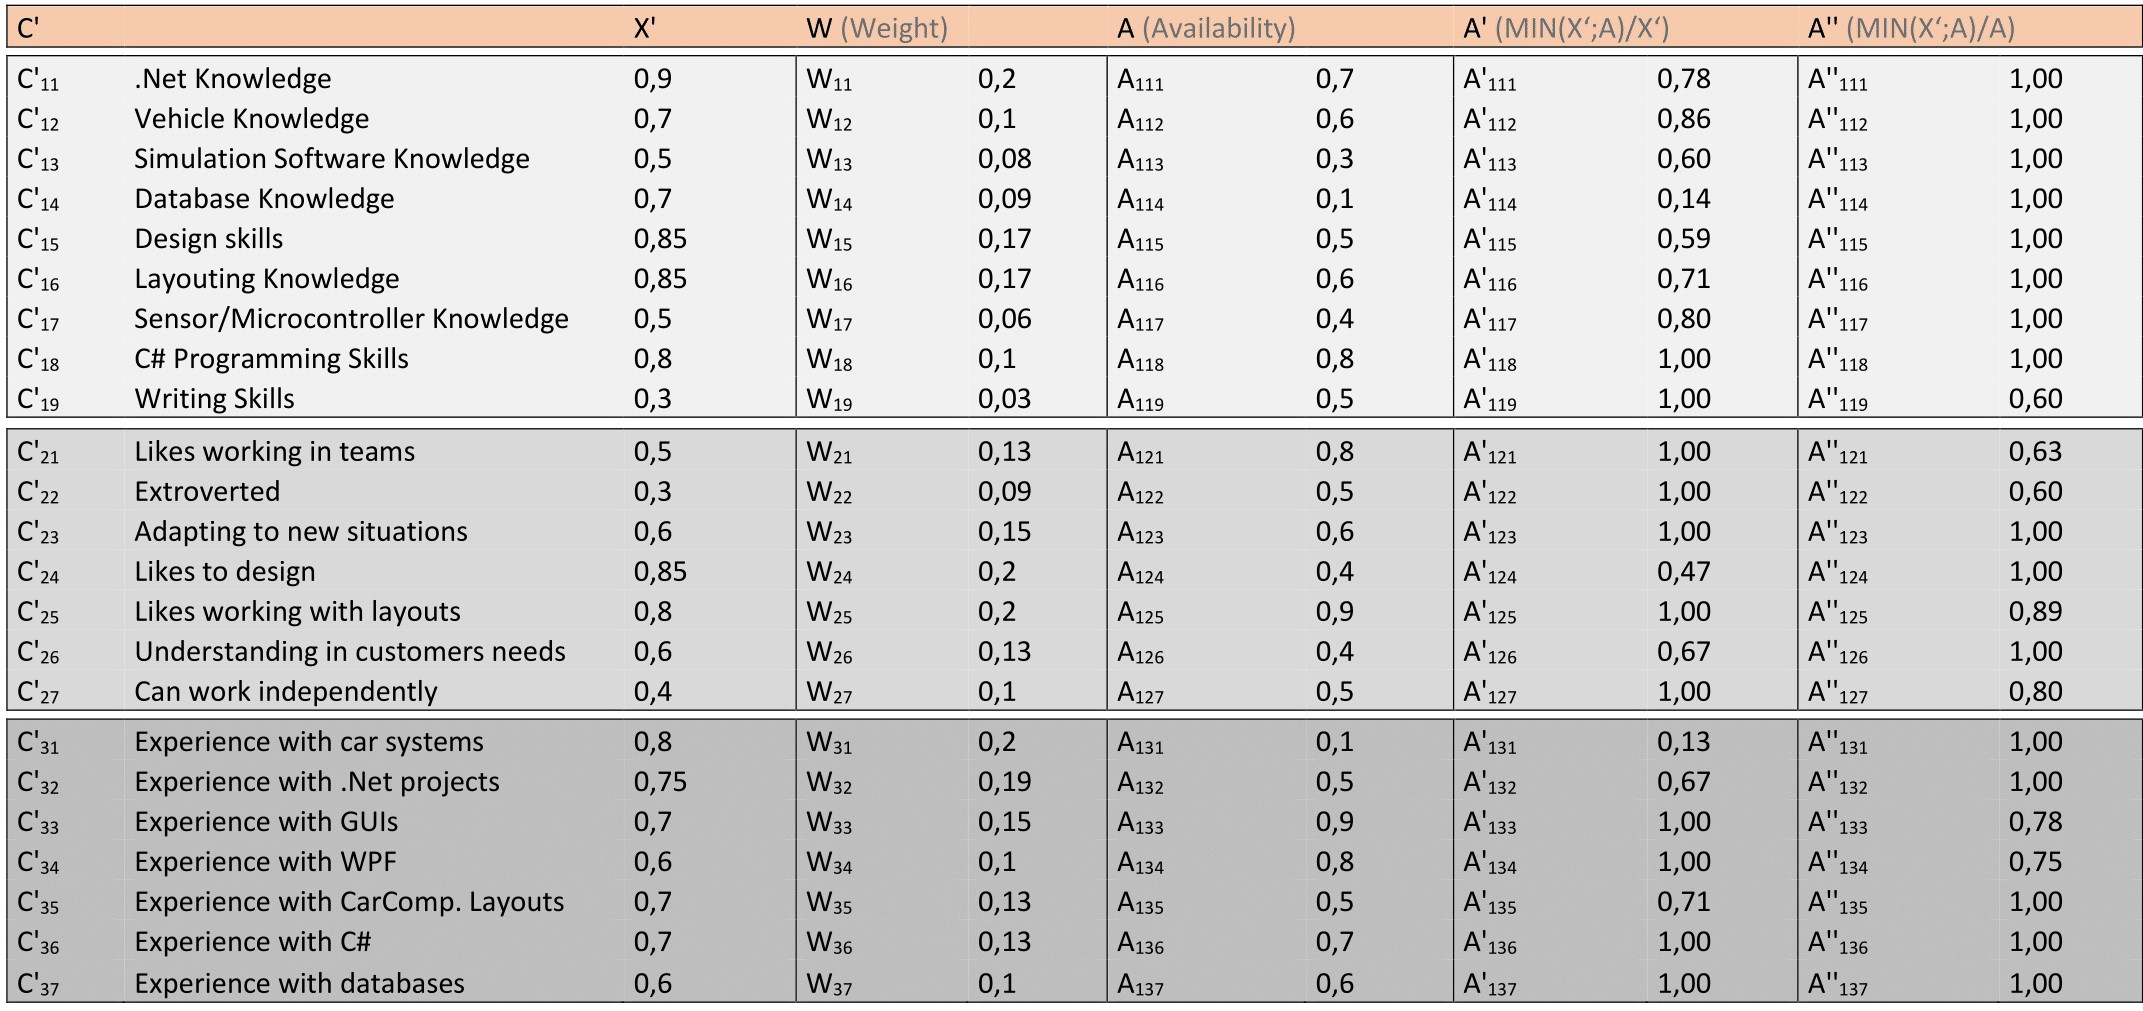
\includegraphics[width=0.75\textheight, angle=90]{res/resAlloc/Table2.jpg}
\caption{Individual Availability}
\label{fig:table2}
\end{figure}

Considering the weight of a skill $W$ and the availability of the human resource
$A$ we can calculate the values $A'$ and $A''$. With those values we can calculate 
the Impact and Utilization of a Human
Resource for a job:

\begin{table}[h]
\centering
\captionsetup{justification=centering}
\begin{tabular}{ll}
\textbf{Impact:} & 0.68 \\
\textbf{Utilisation:} & 0.81
\end{tabular}
\caption{Impact and Utilization of a Human Resource}
\label{tab:ImpactAndUtilization}
\end{table}

\begin{figure}
\centering
\captionsetup{justification=centering}
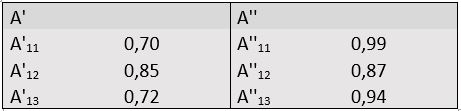
\includegraphics[width=0.75\textwidth]{res/resAlloc/Table3.jpg}
\caption{Normalisation}
\label{fig:table3}
\end{figure}

Those values would have to be compared to the values of other candidates, which
would be too much for this assignment.


\chapter{Risk Analysis}
\vspace{-1cm}
\epigraph{\textbf{Author: } Simon Schneider \newline \textbf{Contributor(s): } }

\vspace{-1cm}
Risk analysis is a process which enables the analysis of risks, associated
within  a project. A Risk can be generally defined as the probability of
something going wrong, and the negative consequences if it does. However, it is
hard to find all the risks, which can occur, in a project. At first it should be
recognised that a risks exists as a consequence of uncertainty. For this reason
the risk analysis process will help to identify potential problems that may
occur. Such a risk analysis can be useful in several situations: 
\begin{itemize}
\item To help to anticipate and neutralise possible problems when planning
projects.
\item To decide wether to continue with the project or not.
\item To improve safety and manage potential risks of the project.
\end{itemize}


\section{Identifying the Risks}
As one of the first steps in Risk Analysis it is to identify the existing and
possible problems occur. Some of these areas and threats, which might have an
impact on this project, are listet below:
\begin{itemize}
\item Project Members -- Illness, injury, or another reason leading to a loss of
a project member.
\item Operational �- Delays in deliveries.
\item Reputational �- Loss of customer or employee confidence.
\item Project �- Taking too long on concluding key tasks, or experiencing
issues with product or service quality, goal not achieved.
\item Financial �- Budget exhausted, Business failure or non-availability of
funding.
\end{itemize}

\section{Estimate Risks}
After some of the possible threats has been faced, the risk can be calculated
with both the likelihood of these threats being realised, and their possible
impact. One way of doing this is to make a estimation of the probability that
this threat occurrs multiplied by the amount it will cost. This leads to the
following equation which quantifies the risk:
\begin{equation}
Risk = Probability\,of\, Occurance \cdot Cost
\end{equation}
Additionally there are two possible kinds of processes:
\begin{itemize}
\item The total value of a risk of a series of processes that are executed
successively can be calculated as follows:
\begin{equation}
R_{Total} = R_{n} \cdot R_{n+1}
\end{equation}
\item The total value of a risk of parallel processes that are executed
concurrent can be calculated as follows:
\begin{equation}
R_{Total} = 1 - (1-R_{n}) \cdot (1 - R_{n+1})
\end{equation}
\end{itemize}

As an example the risk value of an illness of a project member will be
calculated. The estimated propbillity will be set to 0.4. Lets assume that the
member is ill for about a week. One day has 8 working hours and the salary
for this member would be 50\pounds \,per hour. 
\begin{equation}
Risk = Probability\,of\, Occurance \cdot Cost = 0.4 \cdot 5 \cdot 8 \cdot
50\pounds = 800\pounds
\end{equation}
So the risk value for this threat would be 800\pounds. 

In order to determine what risks to focus on, an Impact / Probability Chart can
be very useful. An Impact / Probability Chart is a two dimensional diagram
whereat on the axis of ordinates the probability of Occurrence will be plotted
and on the axis of abscissas the impact on the project. For this purpose, a
probability and the associated impact are assigned to the identified risks.
However, this is carried out only by way of example at a respective risk from
each area and then drawn into the diagram. The assigned probabilities and
impacts can taken from the following table.

\begin{table}[h!]
  \centering
    \footnotesize
\begin{adjustbox}{max width=\textwidth}
\begin{tabular}{c|c|c}
Risk&Probability&Impact\\
\hline
\hline
Illness of Project Member&0.4&3\\
Delay in Deliveries&0.35&8\\
Loss of Customer Confidence&0.5&7\\
Specified Goals not achieved&0.7&9\\
Budget exhausted&0.2&10\\
\end{tabular}
\end{adjustbox}
\captionsetup{justification=centering}
  \caption{Frequency analysis Novel}
  \label{tab:frequency analysis novel}
\end{table}

The following figure shows an exemplarily Impact / Probability Chart with the
estimated probabilities and associated impacts on the project:

\begin{figure}[h!]
  \centering
     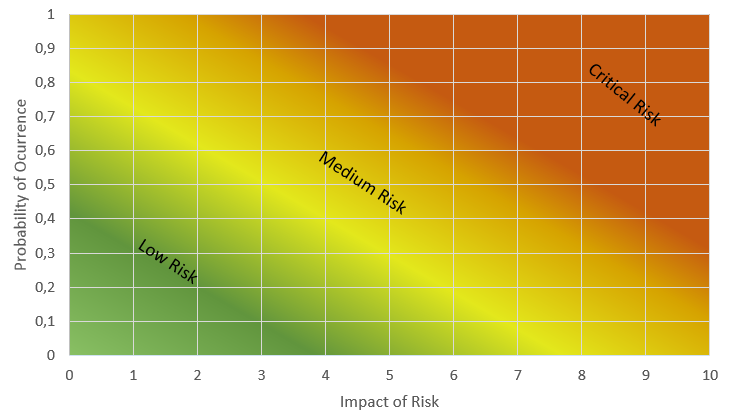
\includegraphics[width=1\textwidth,
     height=0.4\textheight]
     {res/impactchart.png}
     \captionsetup{justification=centering}
  \caption{Impact / Probability Chart}
  \label{fig:ImpactChart}
\end{figure}

\FloatBarrier

As it can be seen, the chart has several areas. With help of this areas it can
be figured out, if the the risk has priority or not. The characteristics of
these areas will be explained subsequently:

\begin{itemize}
\item Low impact/low probability - risks in this area can often be ignored.
\item Low impact/high probability � these risks are of moderate importance but
they have to be noticed and it should be tried to avoid that they occure
\item High impact/low probability - these are of high importance and should not
occure because the probablility is very low. If so, a contingency plans should
be available.
\item High impact/high probability � risks in this area are of critical
importance and have the highest priority.
\end{itemize}

On the basis of this Impact / Probability Chart, the main focus should be on the achievement
of the goals, as these have the highest priority.


\section{Dealing with Risks}

To successfully execute a project, the risks has to be identified. Afterwards
the focus has to be on the middle and high-priority risks. Otherwise resources
on unecessary risks will be a waste. Since the risks has been identified and
prioritised, the next step is how to deal with them. The following is a brief
discussion of four different ways of dealing with risks.

\subsection{Risk Avoidance}
The aim of risk avoidance is to avoid any risk, even if they are very small. The
suggestion of maximum safety through very strong differentiation and a high
control is at the expense of free processes. An example related to the project
is the early planning of the tasks and the associated aims. Through very strict
planning it is already tried in the run-up to avoid all risks, to transfer them
or to turn activities so that risks can not occur. All these actions are at the
expense of project budgets and scheduling but in favor of quality.

The idea of risk avoidance: ``do not take any risks'' means maximum security
while at the same time avoiding opportunities, including rejecting cooperation with
certain partners and a longer project run-time with higher costs.

\subsection{Risk Reduction}
Risk reduction means that through various procedures in the field of personnel
organisation and workplace organisation attempts are made to keep the specific
probability of occurrence of the risks as small as possible. Examples for this
could be, point explicitly to the risks of the respective task to the project
members and communicate the risks transparent to all project members so that a
shared understanding can be achieved.

The idea of risk reduction: by means of personnel processes (training,
qualification, involvement of experts) and technical processes (only processing
quality materials, making processes and optimising them), permanently reduce the
probability of occurrence of risks.

\subsection{Risk Transfer}

During the transfer, risks are passed on to third parties through contracts and
/ or the assignment of service providers. If, for example, many risks occur
during a project phase, it can be considered to outsource the entire task to a
partner.

The idea of risk transfer: through service-level agreements, contracts or
outsourcing, the risks and any related tasks are completely and in writing
passed to third parties, which can then be made liable for a risk entry.

\subsection{Risk Acceptance}
The idea of risk acceptance: risks with very low scope and very low probability
of occurrence, as well as risks that can not be circumvented, should be accepted as such.

\section{Conclusion}
In this chapter it has been worked out what risks are and how they can be
identified. It was then shown how the risk value can be calculated from the
costs and the probability of the occurrence. Afterwards, the identified risks
were prioritized using the Impact / Probability Chart and the handling of risks
was dealt with most recently.

Finally, the further the project progresses, the lower the risk. 

\chapter{Market Analysis}
\vspace{-1cm}
\epigraph{\textbf{Author: } Timo Acquistapace }

\vspace{-1cm}
An important step in the development of a new product is to analyse the market.
This analysis not only includes the identification of competitors and their offered
technologies, but also the investigation of the demand on the product to develop
and its future progression. Another part of the market analysis is to determine
which hardware might be necessary for the product to develop. After the
identification of the needed parts, the offered products on the market are
compared regarding their capabilities and their price.

\section{Analysis of Competitors}
The subsequent analysis is done in an indirect way so that the presented
information is retrieved by querying the internet and putting altogether the
relevant information.

\subsection{Current Systems implemented in today's Cars}
There are only a few systems available that help the driver in leaving a parking
space. These systems exhibit a huge variety of autonomy. The manufacturers
Volvo, Audi and Lincoln sheet park assistance systems that take control over the
steering wheel when leaving a parking lot (see \cite{VolvoCarsSupport},
\cite{Lincoln} and \cite{AudiEspana}). While the steering is done autonomously, 
the driver has to manually operate the pedals.
This kind of systems is mostly restricted to parallel parking.

Mercedes-Benz offers a more autonomous, but also more restricted way of assisted
parking. The �Mercedes Benz Parking Pilot� is able to park and leave the parking
site autonomously. The quitting of the parking site is restricted to those
scenarios in which the Parking Pilot was also used to park the car (see
\cite{DaimlerParkingPilot}).

Tesla offers the Summon functionality implemented in its Model S and Model X. It
allows a driver to leave its car and park as well as retrieve it autonomously.
This feature is restricted to perpendicular parking only (see \cite{TeslaSummon}).

\subsection{Current Systems available from Suppliers}

The development of systems assisting a driver in parking and leaving a parking
lot can be illustrated by the evolution of the products originating from Robert
Bosch GmbH. While the early systems act as it was described for the
manufacturers Volvo, Audi and Bosch (see \cite{Bosch2013}
),
 the current systems are now able to drive itself into and back out of a parking
site autonomously (see \cite{BoschFully}). Another future application of park
assistants is the �Bosch Home Zone Park Assist�. It enables a driver to train its car for certain parking situations
(see 
\cite{BoschHomeZone}).
The car records a route that is driven and it is able to reproduce it even if
the starting point of the route to drive and the one of the recorded route is
slightly different.
On its trained way, the car is able to detect impediments and to react to them.

\subsection{Scientific Projects}
There exist several projects that target on the functionality of autonomously
parking to and leaving from a parking lot.
While the work of Katsev and Braun (see
 \cite{Braun})
 that already started in 2004 seems not to have reached the point where leaving a parking lot is implemented since no further resources can be found on that project,
Roland Doloczki and Don Kevin Gaubitz produced a working prototype of RC-Car
that autonomously leaves a parking space (see
\cite{Doloczki}).
To achieve their goal, Doloczki and Gaubitz use ultrasonic and infrared sensors
to sense the environment around parked vehicle.

\subsection{Development of the market}
It is obvious that the demand on systems that perform certain manoeuvres
autonomously will increase with the success of autonomous cars. But also in the
meantime till these cars make the breakthrough, there might be an increased need
for \acf{ADAS} like parking assistants. Following
McKinsey Inc., there will be three eras in the revolution of self-driving cars
(see \cite{McKinsey}).
The first era, starting from now and lasting till the late 2020s, is
characterised by the first autonomous vehicles being produced and their impact
on established car manufacturers. McKinsey states that the premium makers will
take an incremental approach to autonomous vehicles by implementing more
sophisticated ADAS. This assumption is supported by Statista, assuming that the
shipment of ADAS units will increase by more than 500\% in the time from 2012 to
2020 (see \cite{StatisticaADAS}).

One of the buzz word regarding future driver assistance systems is �Valet
Parking� which means that a car parks itself after the driver has left it and
that the car can be retrieved from its parking position without active control
of the driver. Therefore, Valet Parking needs the possibility of a car
autonomously leaving its parking site. A research project targeting on Valet
Parking was announced by Daimler, Bosch and Car2go in the year 2015 (see
\cite {DaimlerValet}).

\subsection{Conclusion}
It has been worked out that the systems that are implemented in today's cars are
less sophisticated than the system that is planned to develop. Additionally, the
increasing need for ADAS like park assistants has been exposed. However, there
are other scientific projects that aim on the same kind of system and that have
to be overcome by additional functionality or improved safety and reliability.
The major competitor in this sector will be the Robert Bosch GmbH that already
demonstrated its product with a real vehicle and that is working together with a
lot of important car manufacturers like Daimler or Audi.

\section{Market Analysis regarding the needed Hardware}
The product to develop is based on the recognition of obstacles in the vehicle's
surroundings. The most common used sensors to gain an overview of the ambiance
are ultrasonic and laser sensors as well as cameras. Some representatives of
these sensors are presented and compared in this chapter.

\subsection{Comparison of Ultrasonic Distance Sensors }
There exist a lot of ultrasonic distance sensors on the market that are intended
to be used in automotive applications. The chosen representatives of these all
exhibit a detection range of $1m$ or above. Their switching frequency, operation
temperature and price are compared in table \ref{tab:ultrasonic}.

\begin{table}
\centering
\captionsetup{justification=centering}
\footnotesize
\renewcommand{\arraystretch}{1.5}
\begin{tabular}{p{0.3\textwidth}|p{0.35\textwidth}|p{0.1\textwidth}|p{0.1\textwidth}}
Product & Key Features & Price & Retailer \\
\hline
SICK UM18-218161101 
& Range: 0.12 - 1.0m \newline 
	operation temp.: -25\degree C - 70\degree C \newline 
	Switching freq.: 10Hz 
& 152.32\$ 
& \cite{tme} \\
PING))) Ultrasonic Distance Sensor 
& Range: 0.02 - 3m \newline 
	operation temp.: 0\degree C - 70\degree C  \newline 
	Switching freq.: 10Hz 
& 24.99\$ 
& \cite{parallax}\\
LV-MaxSonar-EZ1 
& Range: 0.0 - 6.45m\newline 
	operation temp.: -  \newline 
	Switching freq.: 20Hz  
& 23.36\$ 
& \cite{sparkfun} \\
AU003 
& Range: 0.08 - 1.2m\newline 
	operation temp.: -20 \degree C - 70 \degree C  \newline 
	Switching freq.: 5Hz  
& 112.94\$ 
& \cite{autosen} \\
\end{tabular}
\caption{Compared Ultrasonic Distance Sensors}
\label{tab:ultrasonic}
\end{table}

While the low-cost sensors are appropriate for a proof of concept, they are not
suitable for an application under real conditions because either their operation
temperature lies only above freezing or it is not indicated in the datasheets.
The prices of the high-cost sensors are based on the ordering of small amounts
and might be renegotiated if higher volumes are commissioned.

\section{Comparison of Laser Distance Sensors}
Laser distance sensors are especially popular in the context of the obstacle
detection that is implemented by Google's self-driving car (see \cite{whitwam}).
Different representatives of this kind of sensor are contrasted in table
\ref{tab:laser}.
\begin{table}
\centering
\captionsetup{justification=centering}
\footnotesize
\renewcommand{\arraystretch}{1.5}
\begin{tabular}{p{0.3\textwidth}|p{0.35\textwidth}|p{0.1\textwidth}|p{0.1\textwidth}}
Product & Key Features & Price & Retailer \\
\hline
OID200 - OIDLCPKG/US
& Range: 0.03 - 2.0m \newline 
	operation temp.: -25\degree C - 60\degree C \newline 
	Switching freq.: 11Hz 
& 115.69\$ 
& \cite{automation24} \\
Lidar Lite v3
& Range: up to 40m \newline 
	operation temp.: -20\degree C - 60\degree C  \newline 
	Switching freq.: 10Hz 
& 159.15\$ 
& \cite{sparkfun2}\\
AL003 
& Range: 0.03 � 2m\newline 
	operation temp.: -25\degree C - 60\degree C \newline 
	Switching freq.: 11Hz  
& 110.05\$ 
& \cite{autosen2} \\
\end{tabular}
\caption{Compared Laser Distance Sensors}
\label{tab:laser}
\end{table}

All of the presented sensors are designed for the use in automotive applications
and therefore fulfil the requirements for our project. In contrast to the
ultrasonic sensors, there are no low-cost laser distance sensors that are
suitable for the use in a proof of concept.

\subsection{Review on available Camera Sensors}
Comparing available camera sensors on the market is very difficult. Most of the
available sensors are designed to be used in model making. The prices of the
ones that are intended for automotive applications (e.g. sensors of Ambarella
and ON Semiconductor) have to be inquired from the manufacturers. Table
\ref{tab:camera} shows two camera sensors that are suitable for a proof of
concept that could also be tested under the condition of extreme temperatures.

\begin{table}
\centering
\captionsetup{justification=centering}
\footnotesize
\renewcommand{\arraystretch}{1.5}
\begin{tabular}{p{0.3\textwidth}|p{0.35\textwidth}|p{0.1\textwidth}|p{0.1\textwidth}}
Product & Key Features & Price & Retailer \\
\hline
32KM NTSC
& Resolution: 0.35MP \newline 
	operation temp.: -20\degree C - 70\degree C \newline 
	Scanning freq.: 60Hz, \newline
	night vision: no, \newline
	angle: up to 120\degree
& 31.95\$ 
& \cite{sparkfun3} \\
LinkSprite JPEG Color Camera TTL Interface - Infrared
& Resolution: 0.3MP \newline 
	operation temp.: -20\degree C - 70\degree C \newline 
	Scanning freq.: 60Hz, \newline
	night vision: yes, \newline
	angle: up to 120\degree
& 49.95\$ 
& \cite{sparkfun4}
\end{tabular}
\caption{Sampled Camera Sensors}
\label{tab:camera}
\end{table}

\subsection{Calculation of Costs}
If a hardware proof of concept is implemented, the costs can be calculated like
it is done in table \ref{tab:costs}. The amount of sensors that are used in a
final system and the actual prices might differt in the moment of the
system's realisation.

\begin{table}
\centering
\captionsetup{justification=centering}
\renewcommand{\arraystretch}{1.5}
\begin{tabular}{llll}
Part & Price/Unit & Pcs & Sum \\
\hline
32KM NTSC & 31.95\$ & 2 & \hspace{0.07cm} 63.90\$ \\
LV-MaxSonar-EZ1 & 23.36\$ & 4 & \hspace{0.07cm} 93.44\$ \\
 Arduino Mega 2560 & 37.18\$ & 1 & \hspace{0.07cm} 37.18\$ \\ 
\hline
Total & & & 194.52\$
\end{tabular}
\caption{Calculation of Costs for a POC}
\label{tab:costs}
\end{table}
 

\chapter{Process Flow, Critical Path Identification and Predictive Models}
\vspace{-1cm}
\epigraph{\textbf{Author: } Markus Just}

\chapter{Customer Reports and Analysis}
\vspace{-1cm}
\epigraph{\textbf{Author: } Timo Acquistapace }

\vspace{-1cm}
Giving the customer the possibility to participate in the development of a
product by providing him transparency regarding the overall progress and by 
implementing its feedback is one of the most important success factors.
Especially if the final results of the collaboration are not explicitly clear or
if the project is some kind of research work, it is of highest importance to
gather the customer's feedback continuously. The gained feedback serves as an
input in adapting the product or even the whole process of development.

\begin{figure}
\centering
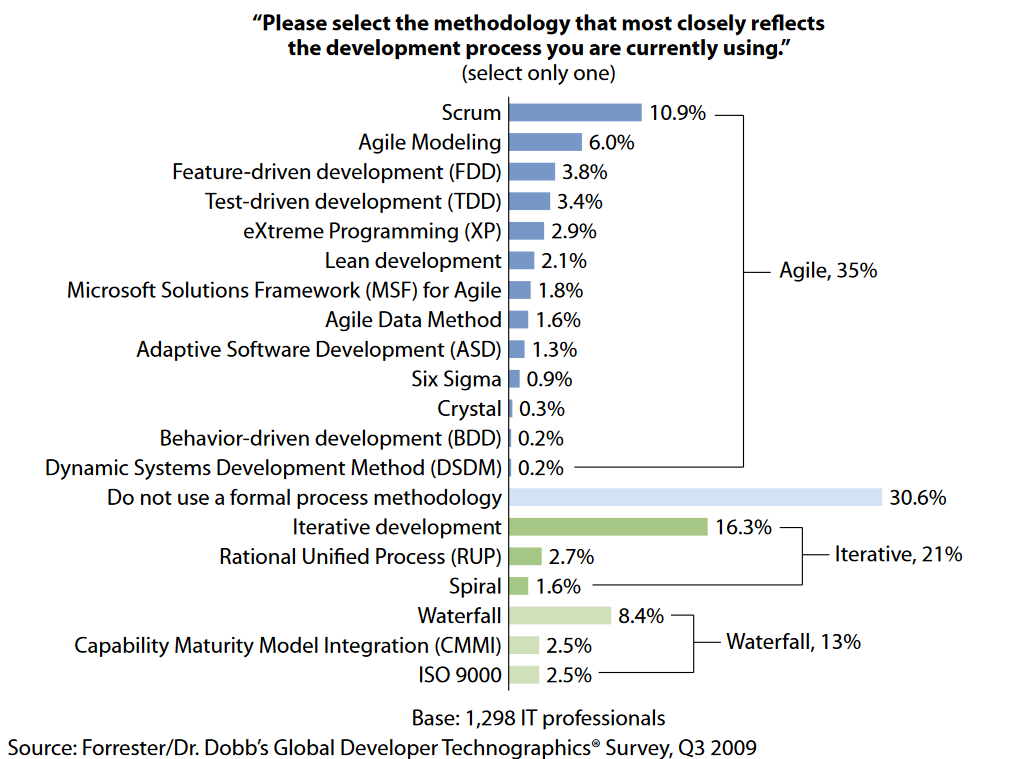
\includegraphics[width=0.75\textwidth]{res/customerVoice/applicationOfAgileMethods.PNG}
\caption{Adoption of agile Methods in Software Development (\cite{forrester})}
\label{fig:agileAdoption}
\end{figure}

Especially in the area of software development, the need for constant
interaction between a manufacturer and its customer is widely acknowledged. This
fact can be demonstrated by the adoption of agile methods (see figure
\ref{fig:agileAdoption}). These methods, like XP, Scrum and FDD, offer the
possibility of high transparency, short feedback-cycles and increased
flexibility regarding changes in the requirements or in the market -�
characteristics that proved themselves good and that are strongly wanted 
by the manufacturers adopting agile methods (see figure
\ref{fig:agileFeatures}).

\begin{figure}
\centering
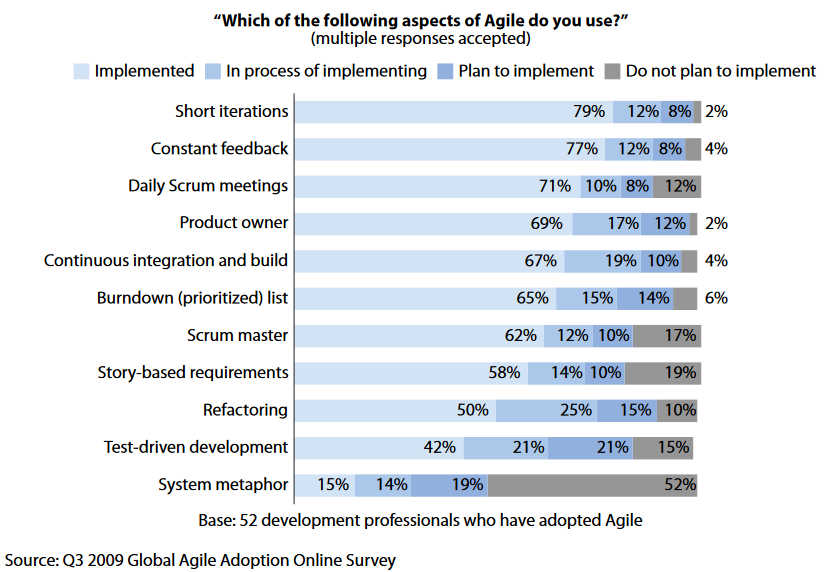
\includegraphics[width=0.75\textwidth]{res/customerVoice/aspectsOfAgile.PNG}
\caption{Adoption of agile Methods in Software Development (\cite{forrester})}
\label{fig:agileFeatures}
\end{figure}

\section{Determining the Modalities of Collaboration}
\label{sect:firstQuestionnaire}
To embed a process that as well satisfies the customer as it provides the
manufacturer the possibility to get as much useful input and feedback as
possible, the modalities of collaboration are negotiated as a first step. The
salient points in this negotiation are:

\begin{itemize}
\item{Who is the customer's specialist contact person and how should the
communication with him/her take place?}
\item{Who is the customer's technical contact person and how should the
communication with him/her take place?}
\item{In which way will the customer contact our company if necessary?}
\item{What are the customers preferences regarding the reports on the project's progress?}
\end{itemize}

While some of these points like the contact information of a certain person in
charge are only of informational kind, other points like the desired way of
communication are of high importance. Since there are certain preferences in our
company regarding the length of the iterations and the way how the communication
should take place, the CORE value of the customer's answers in respect of our
company's preferences is calculated.

\subsection{Results}
The results of the first questionnaire that serves to determine the modalities
of collaboration between our company and our customer are presented in this
section. The analysis of the results can be found in section
\ref{sect:q1_results}. Answers that contain personal data like contact
information are omitted.

\begin{figure}
\centering
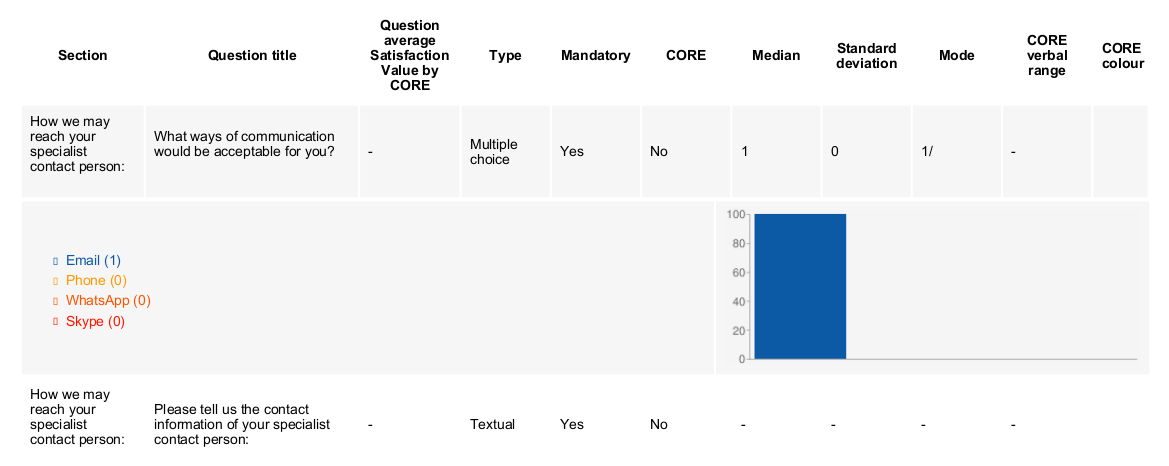
\includegraphics[width=\textwidth]{res/customerVoice/q1_results/q1.png}
%\caption{Overview of first Questionnaire's Results}
%\label{fig:resultsOverview}
\end{figure}

\begin{figure}
\centering
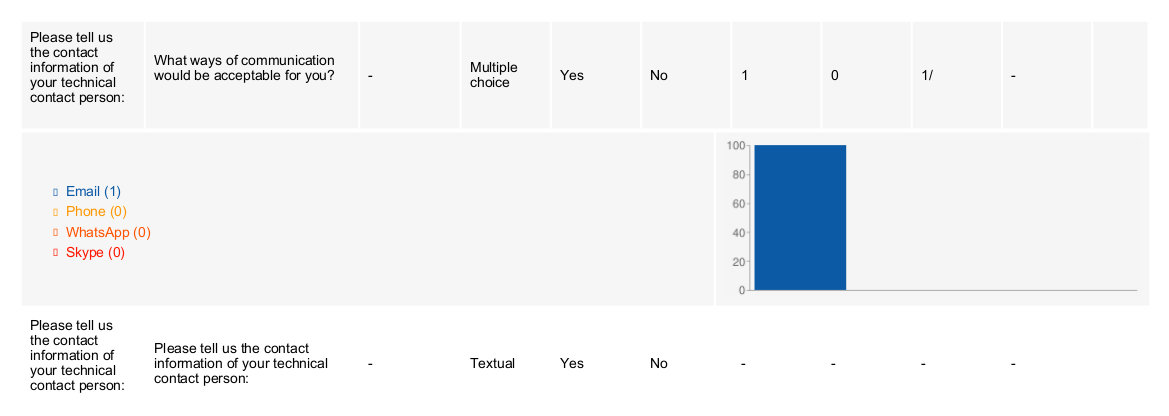
\includegraphics[width=\textwidth]{res/customerVoice/q1_results/q2.png}
%\caption{Overview of first Questionnaire's Results}
%\label{fig:resultsOverview}
\end{figure}

\begin{figure}
\centering
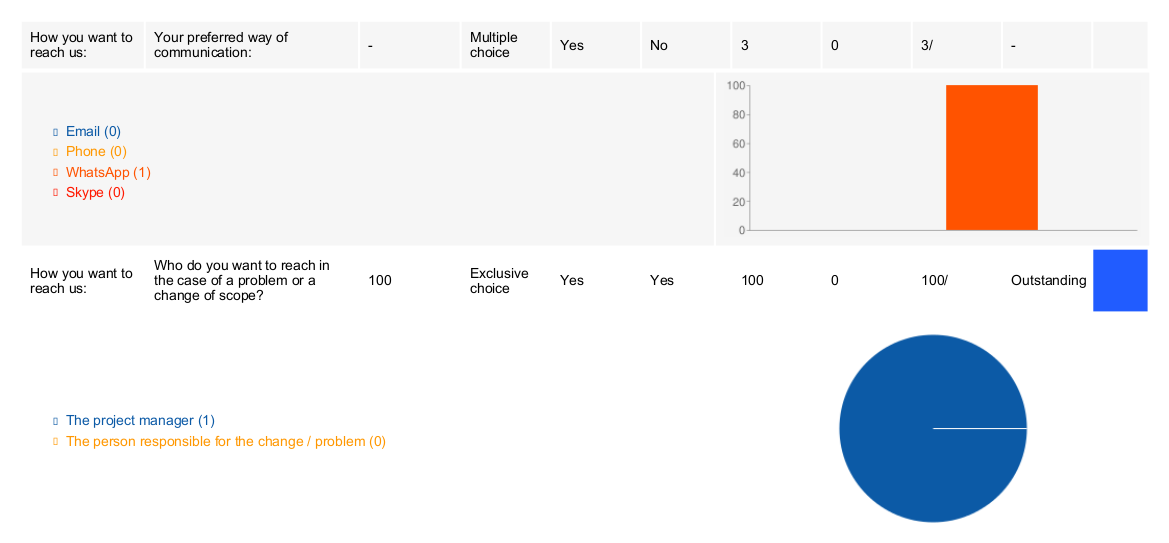
\includegraphics[width=\textwidth]{res/customerVoice/q1_results/q3.png}
%\caption{Overview of first Questionnaire's Results}
%\label{fig:resultsOverview}
\end{figure}

\begin{figure}
\centering
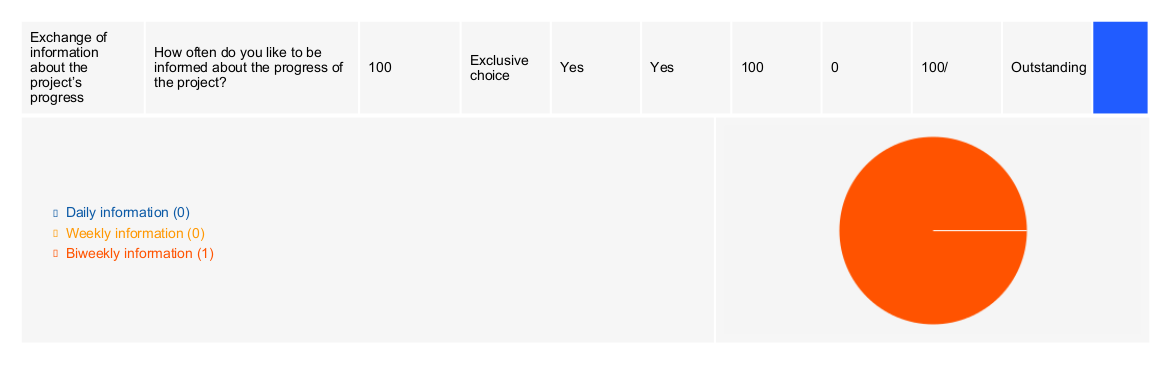
\includegraphics[width=\textwidth]{res/customerVoice/q1_results/q4.png}
%\caption{Overview of first Questionnaire's Results}
%\label{fig:resultsOverview}
\end{figure}

\begin{figure}
\centering
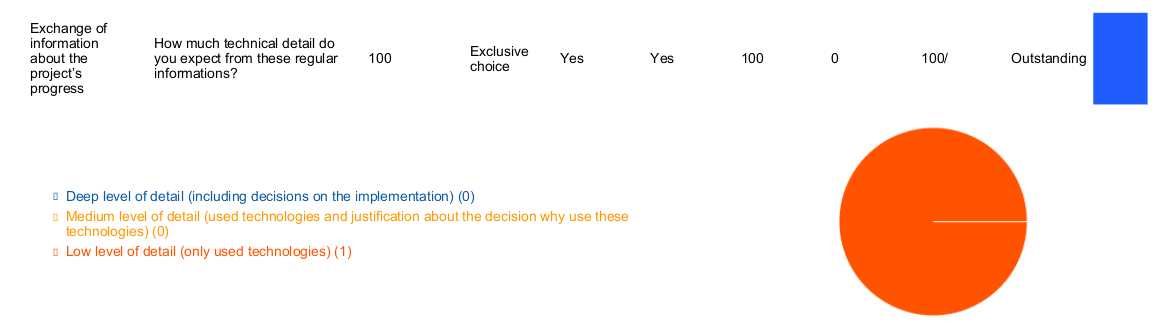
\includegraphics[width=\textwidth]{res/customerVoice/q1_results/q5.png}
%\caption{Overview of first Questionnaire's Results}
%\label{fig:resultsOverview}
\end{figure}

\begin{figure}
\centering
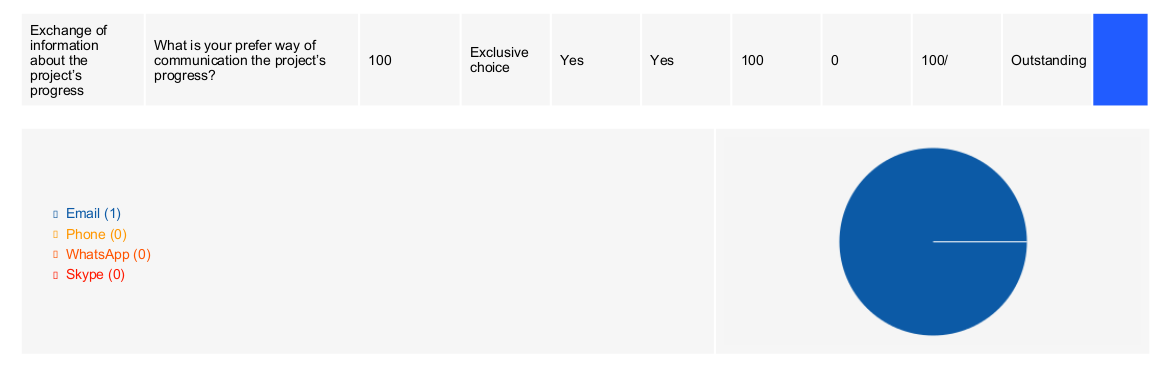
\includegraphics[width=\textwidth]{res/customerVoice/q1_results/q6.png}
%\caption{Overview of first Questionnaire's Results}
%\label{fig:resultsOverview}
\end{figure}

\begin{figure}
\centering
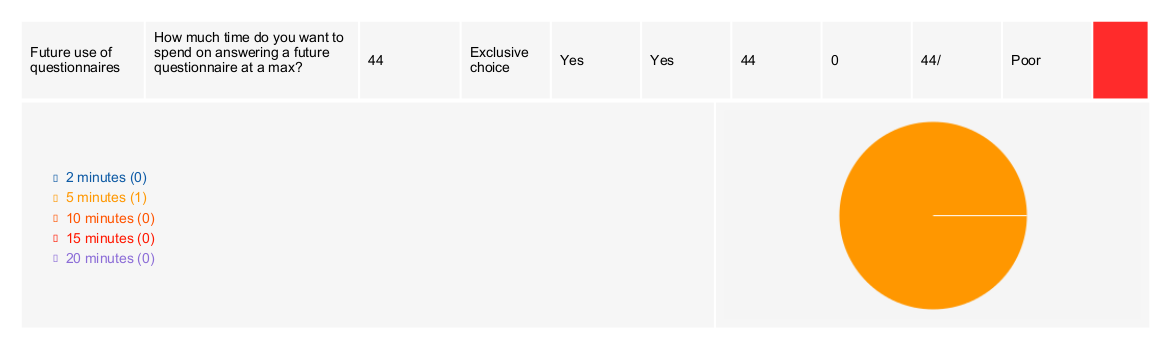
\includegraphics[width=\textwidth]{res/customerVoice/q1_results/q7.png}
%\caption{Overview of first Questionnaire's Results}
%\label{fig:resultsOverview}
\end{figure}

\begin{figure}
\centering
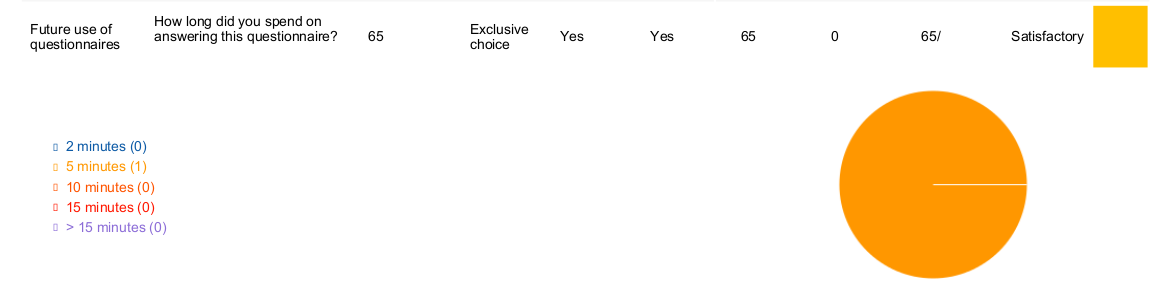
\includegraphics[width=\textwidth]{res/customerVoice/q1_results/q8.png}
%\caption{Overview of first Questionnaire's Results}
%\label{fig:resultsOverview}
\end{figure}

\begin{figure}
\centering
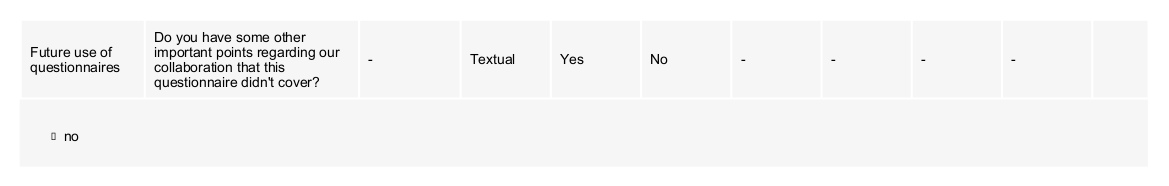
\includegraphics[width=\textwidth]{res/customerVoice/q1_results/q9.png}
%\caption{Overview of first Questionnaire's Results}
%\label{fig:resultsOverview}
\end{figure}

\FloatBarrier
\subsection{Gained Knowledge}
\label{sect:q1_results}

\begin{figure}
\centering
\captionsetup{justification=centering}
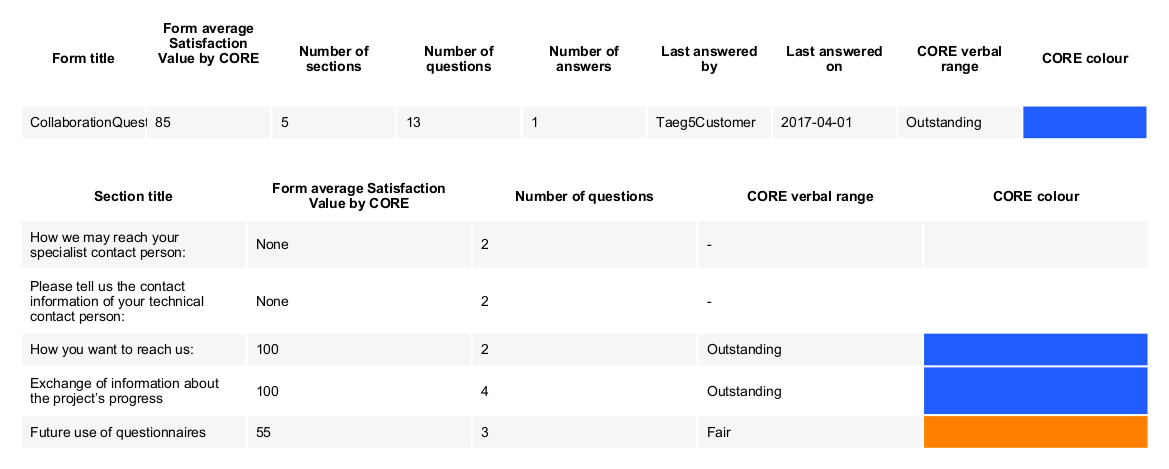
\includegraphics[width=\textwidth]{res/customerVoice/q1_results/overview.png}
\caption{Overview of first Questionnaire's Results}
\label{fig:resultsOverview}
\end{figure}

The result of the questionnaire is as well important as it is satisfactory to
our company since the most answers given by the customer reflect the preferences
of our company. This is especially true regarding the questions on the way our
company will contact the customer, on the interval that is used for reporting
and on the reporting's level of detail.

While the fact that our customer wants to contact the project manager and not
any other team member complies with our company's preferences, the way of
contacting him is suboptimal in our opinion. Nevertheless, our company will
attend the customer's wished in this point.

To be able to gain honest and serious feedback from following questionnaires and
not to overstrain our customer's willingness to collaborate, the last section
deals with questionnaires in general. It is determined how long it took to
answer the current questionnaire and how much time our customer is willing to
spent in answering future questionnaires. For the simple reason that it was
estimated that answering the current questionnaire would take 10 minutes, the
CORE value retrieved from the answers on these questions is not highest
achievable value. However, the result shows that the questionnaire's length
perfectly fit the customer's preferences. Future questionnaires will therefore
be designed in a way that they nearly have the same length and the CORE values
for the options on the question how long it took to answer a questionnaire 
will be adapted.

\section{Clarification of the Requirements and Assessment of the first Design}
Prototype Gathering and writing down requirements for a product requires high
prudence. \cite{Young} defines 15 characteristics of good requirements. Even if
high effort is expended in the process of requirements engineering, there are
mostly requirements that don't exhibit all of these characteristics. In the most
cases, these requirements lack clarity and expressiveness.

The unclear requirements as well as a first mockup are the basis of a second
questionnaire. Its aims are to inform the customer how the vague requirements
were interpreted in the first step, to offer the customer the possibility to
give a feedback on this interpretation and to provide him a first sense of the
product that will be developed. The mockup that was created for the purpose of
this questionnaire is depicted in figure \ref{fig:initialMockup}.

\begin{figure}
\centering
\captionsetup{justification=centering}
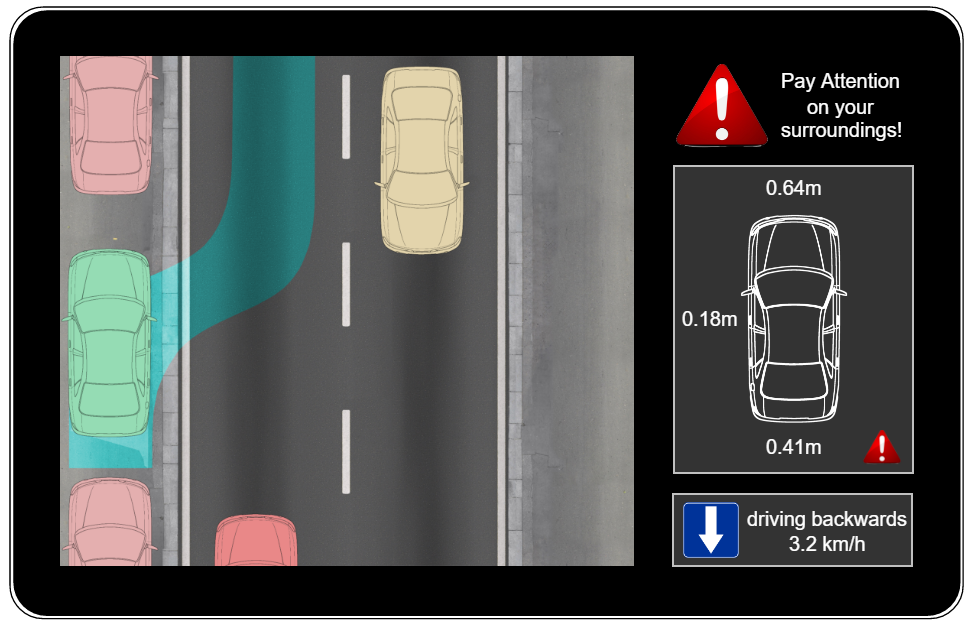
\includegraphics[width=0.75\textwidth]{res/customerVoice/mockup.png}
\caption{Initial Mockup of the System}
\label{fig:initialMockup}
\end{figure}

\subsection{Results}
The results that help to clarify the requirements and to get a first feedback on
the planned design are depicted below and interpreted in the next section (see
section \ref{sect:q2_results}). Since a mistake has been made on the creation of
the questionnaire, the assessment how long it took the customer to answer it had
to be done in an additional form. The results of the initial survey and the
additional form are assembled together.

\begin{figure}[h!]
\centering
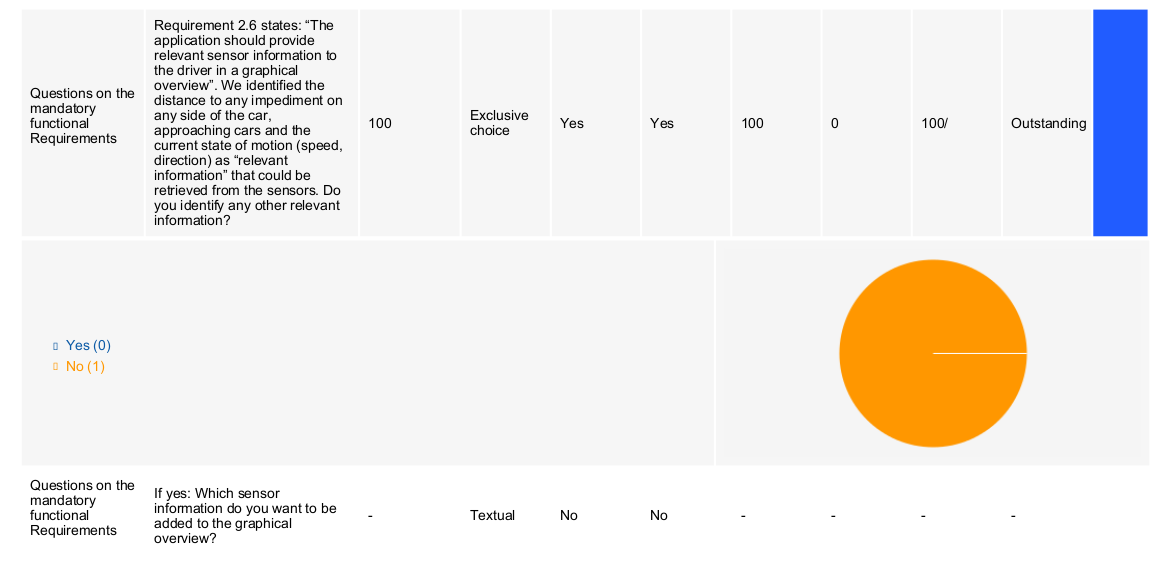
\includegraphics[width=\textwidth]{res/customerVoice/q2_results/q1.png}
%\caption{Overview of first Questionnaire's Results}
%\label{fig:resultsOverview}
\end{figure}

\begin{figure}
\centering
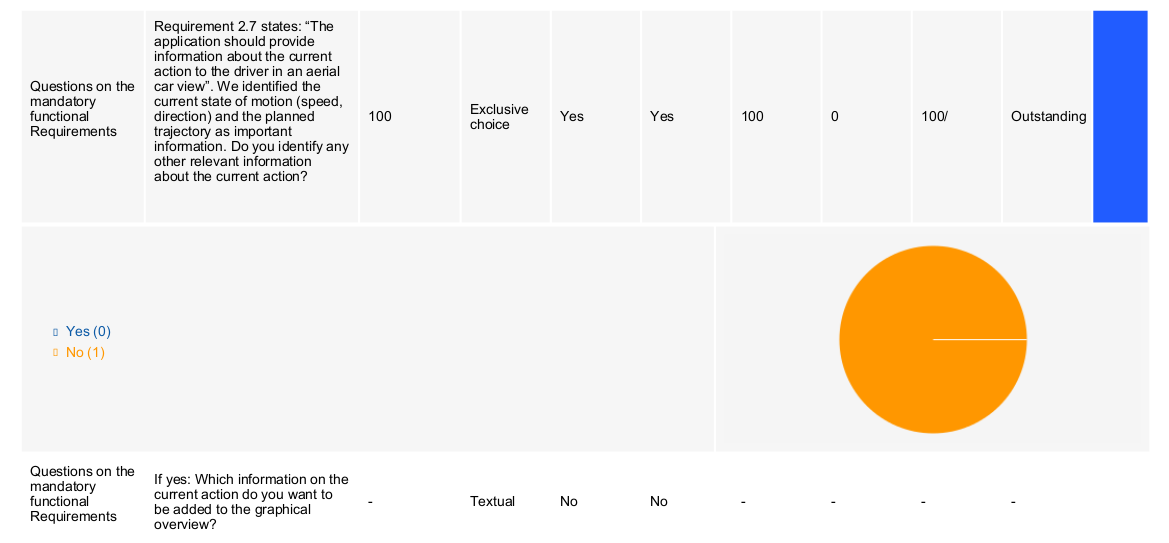
\includegraphics[width=\textwidth]{res/customerVoice/q2_results/q2.png}
%\caption{Overview of first Questionnaire's Results}
%\label{fig:resultsOverview}
\end{figure}

\begin{figure}
\centering
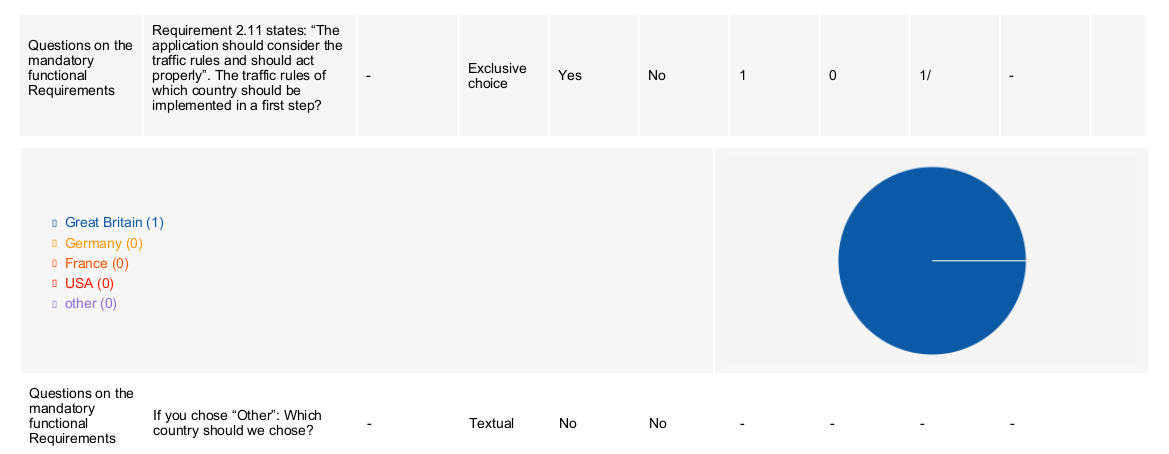
\includegraphics[width=\textwidth]{res/customerVoice/q2_results/q3.png}
%\caption{Overview of first Questionnaire's Results}
%\label{fig:resultsOverview}
\end{figure}

\begin{figure}
\centering
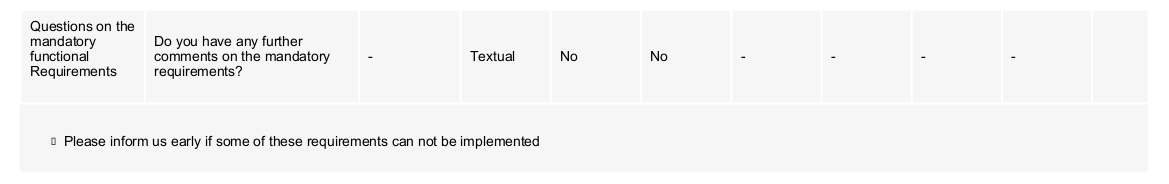
\includegraphics[width=\textwidth]{res/customerVoice/q2_results/q4.png}
%\caption{Overview of first Questionnaire's Results}
%\label{fig:resultsOverview}
\end{figure}

\begin{figure}
\centering
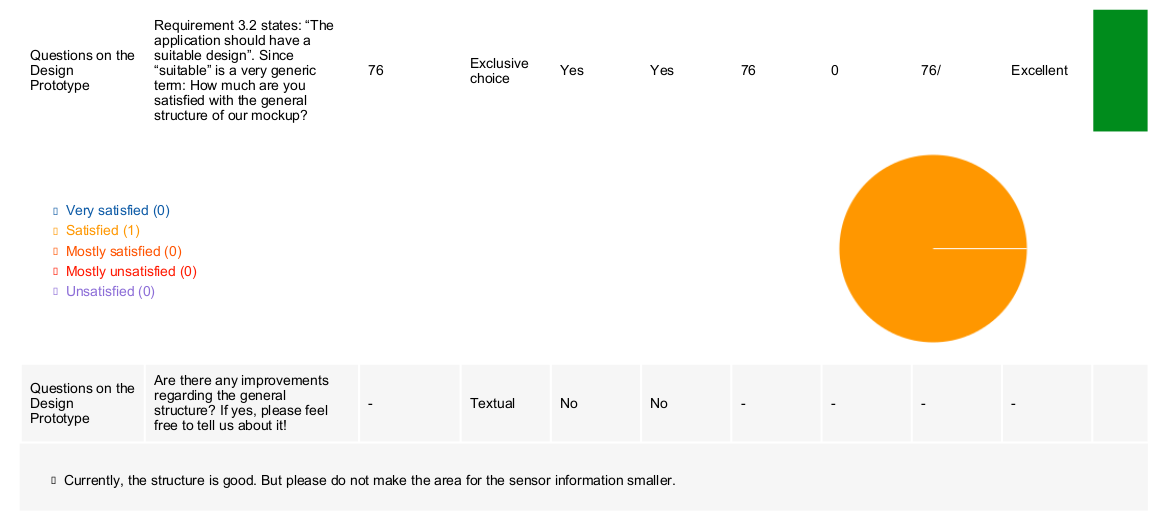
\includegraphics[width=\textwidth]{res/customerVoice/q2_results/q5.png}
%\caption{Overview of first Questionnaire's Results}
%\label{fig:resultsOverview}
\end{figure}

\begin{figure}
\centering
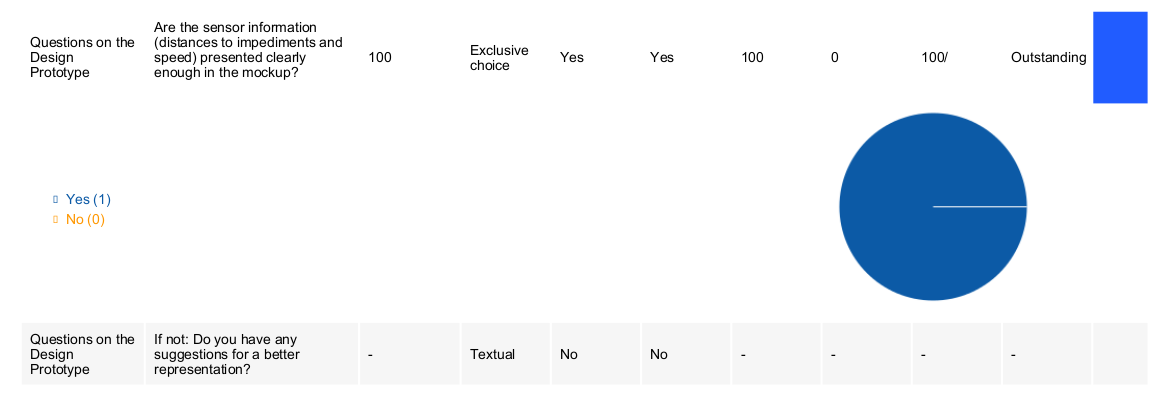
\includegraphics[width=\textwidth]{res/customerVoice/q2_results/q6.png}
%\caption{Overview of first Questionnaire's Results}
%\label{fig:resultsOverview}
\end{figure}

\begin{figure}
\centering
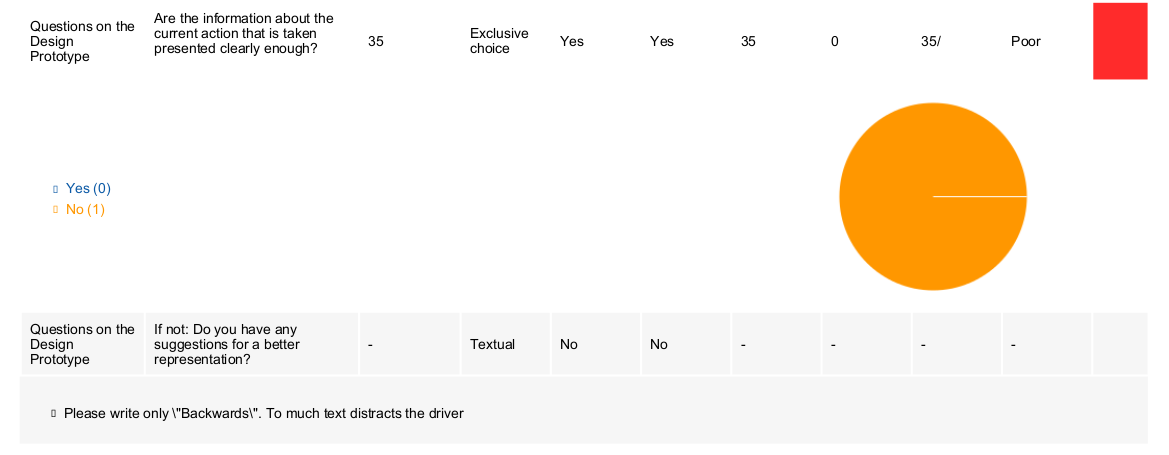
\includegraphics[width=\textwidth]{res/customerVoice/q2_results/q7.png}
%\caption{Overview of first Questionnaire's Results}
%\label{fig:resultsOverview}
\end{figure}

\begin{figure}
\centering
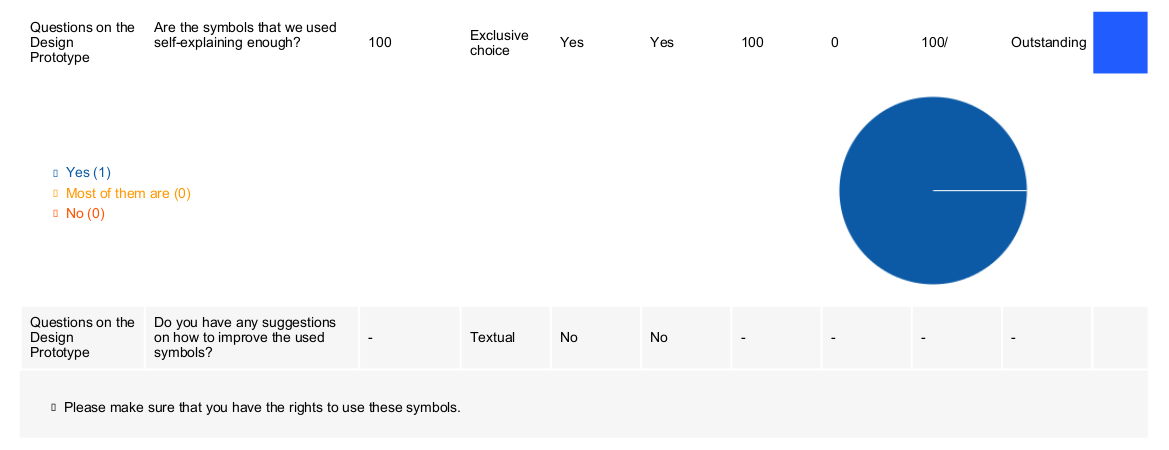
\includegraphics[width=\textwidth]{res/customerVoice/q2_results/q8.png}
%\caption{Overview of first Questionnaire's Results}
%\label{fig:resultsOverview}
\end{figure}

\begin{figure}
\centering
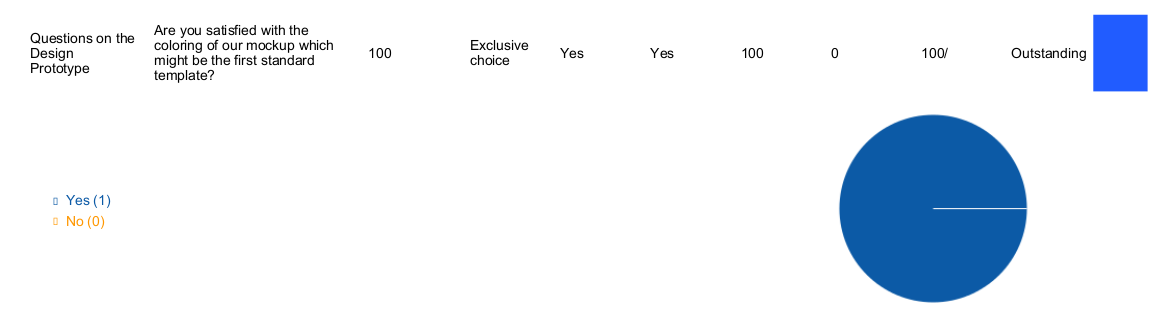
\includegraphics[width=\textwidth]{res/customerVoice/q2_results/q9.png}
%\caption{Overview of first Questionnaire's Results} 
%\label{fig:resultsOverview}
\end{figure}

\begin{figure}
\centering
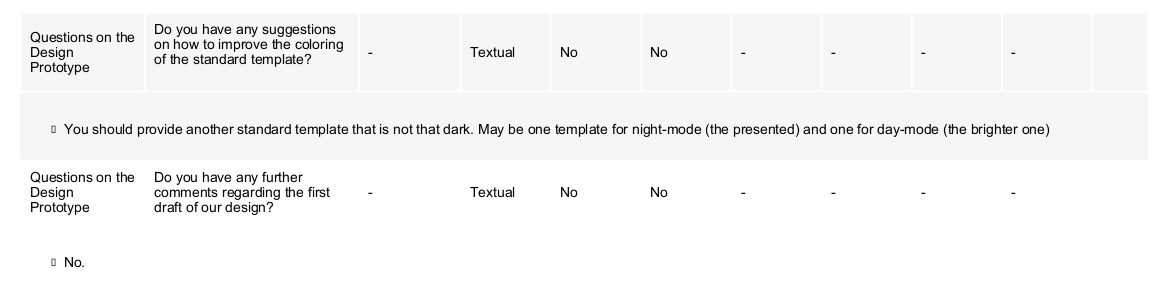
\includegraphics[width=\textwidth]{res/customerVoice/q2_results/q10.png}
%\caption{Overview of first Questionnaire's Results}
%\label{fig:resultsOverview}
\end{figure}

\begin{figure}
\centering
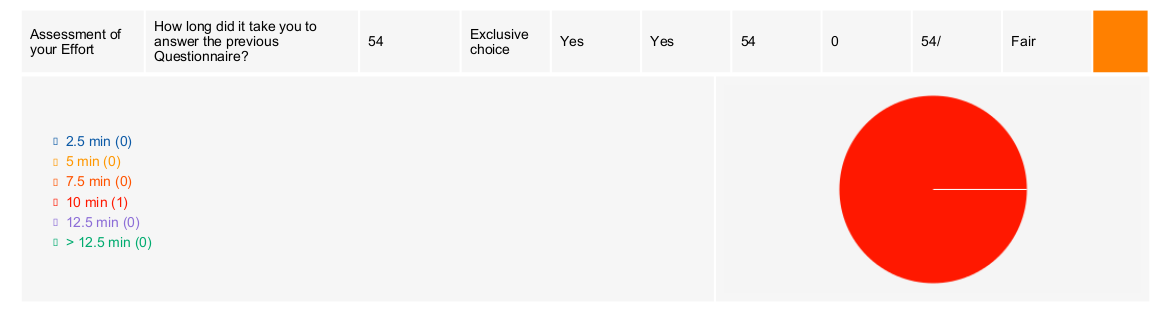
\includegraphics[width=\textwidth]{res/customerVoice/q2_results/q11.png}
%\caption{Overview of first Questionnaire's Results}
%\label{fig:resultsOverview}
\end{figure}

\FloatBarrier

\subsection{Gained Knowledge and further Steps taken}
\label{sect:q2_results}

\begin{figure}
\centering
\captionsetup{justification=centering}
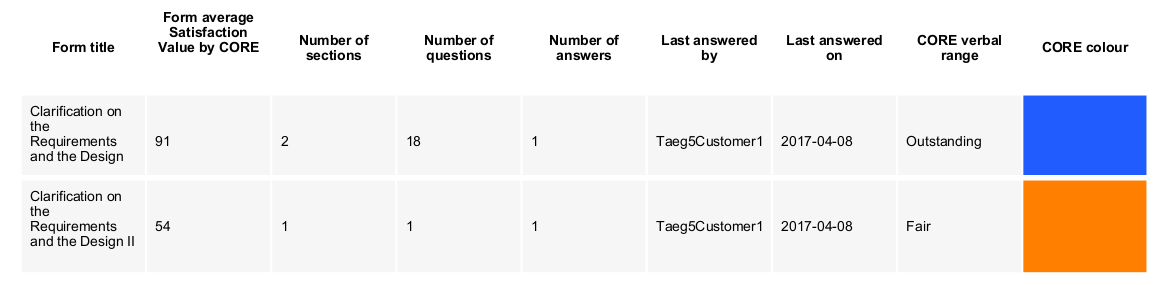
\includegraphics[width=\textwidth]{res/customerVoice/q2_results/overview.png}
\caption{Overview of second Questionnaire's Results}
\label{fig:resultsOverview2}
\end{figure}

As it can be seen in \ref{fig:resultsOverview2}, the results are very satisfying
and the interpretation of the requirements fits the customer's expectations.
More detailed feedback could be gathered regarding the design of the system. In
the further development, our company will focus its attention to simplify the
design e.g. by shortening the presented texts and by trying to scale up the area
that presents the sensor information.

Unfortunately, the customer was not able to answer the questionnaire within 5
minutes as preferred, although the open questions on the optional requirements
were already omitted. Since this was expected and the clarification of the
requirements is a very important point, it is acceptable in the case of the
current survey. Nevertheless, there has to be some effort made in the future to
keep the questionnaires as short as possible for not deceiving the customer
again in this regard.

\section{Interim Report about the Project's Progress}
As it was determined in the first questionnaire (see section 
\ref{sect:firstQuestionnaire}), our customer wishes to get biweekly information
about the project's current progress. The information included should exhibit a
low level of technical detail and only reflect the relevant design decisions. A
sample report can be found in the following pages.

\FloatBarrier

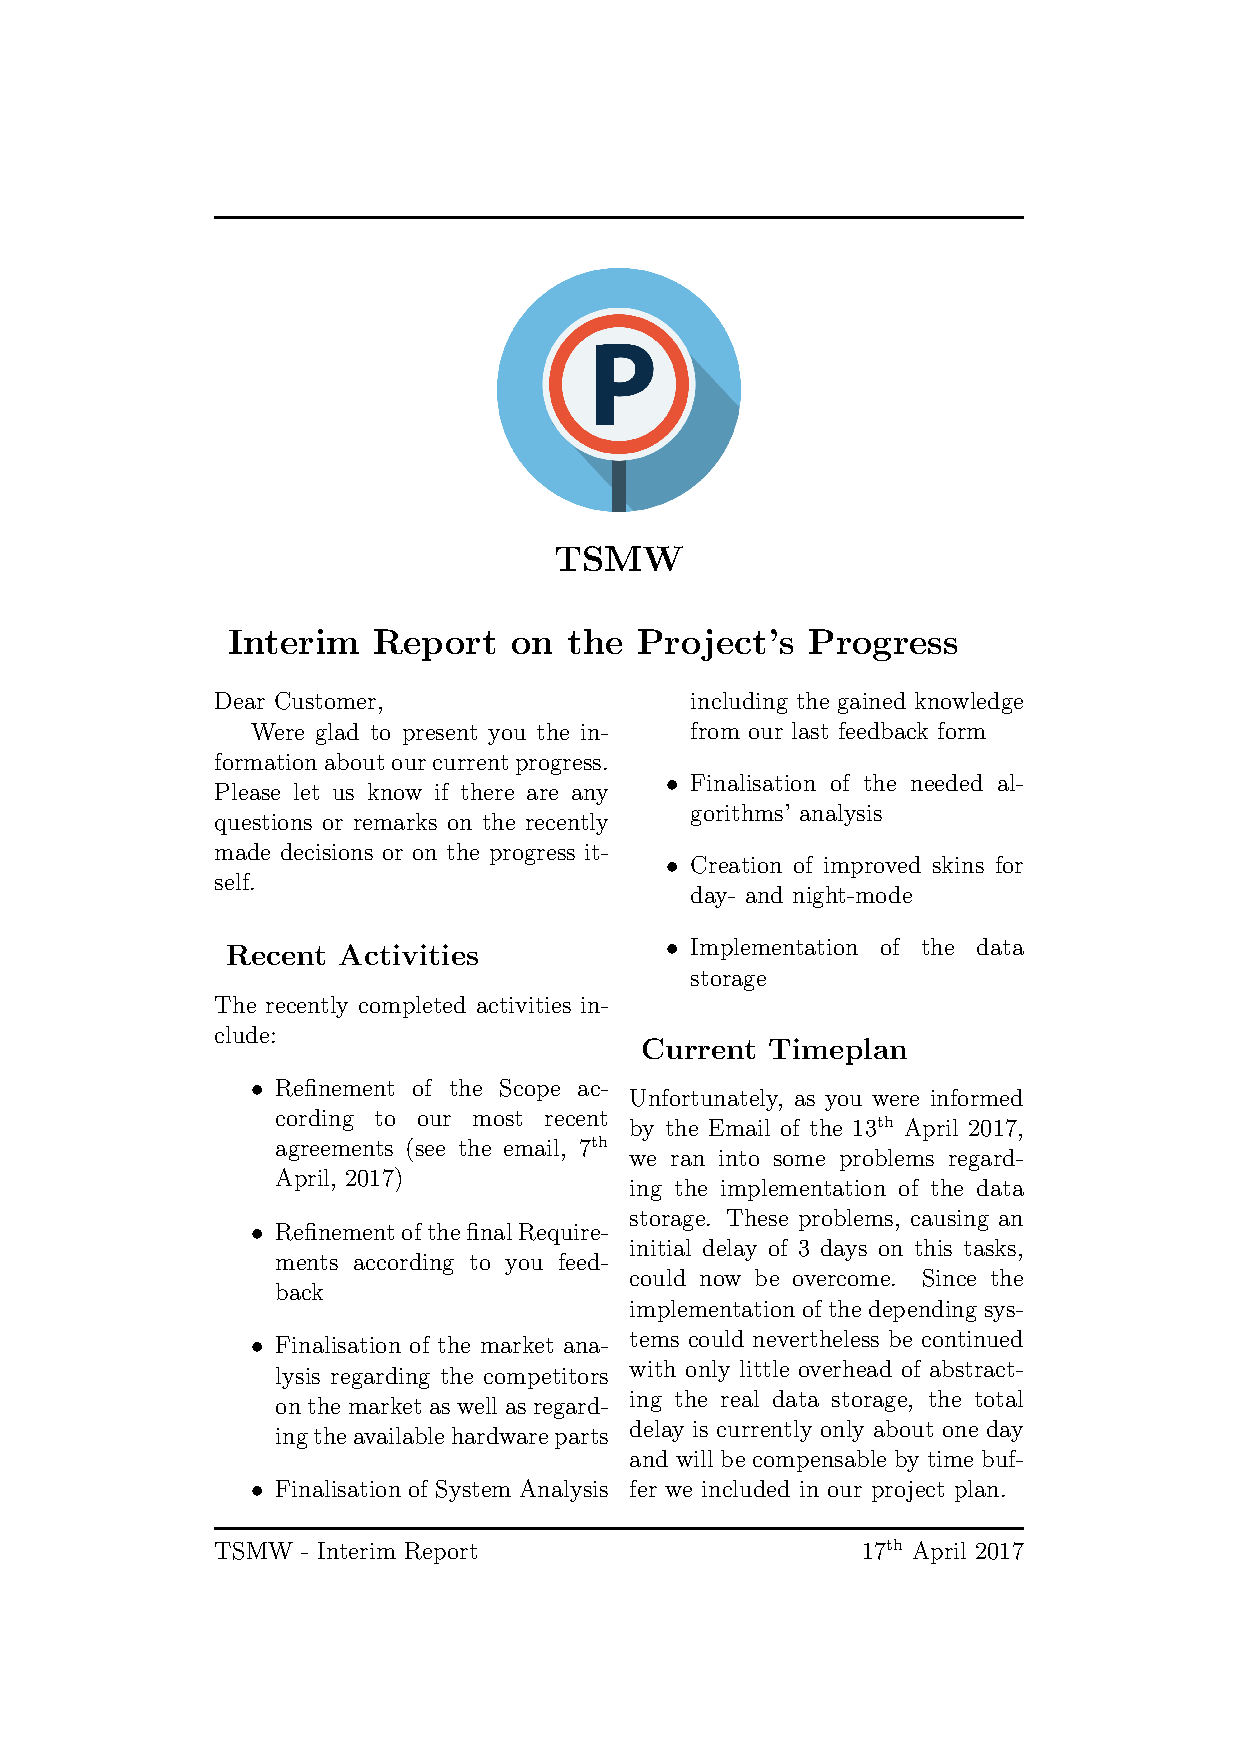
\includepdf[pages={-}]{res/customerVoice/interimReport/interimReport.pdf}

\section{Final Evaluation of the customers satisfaction}
Up to this point, Satistica was mainly used to clarify open questions. After the
termination of the project, it is important to determine the customer's
satisfaction. This determination enables our company to perform
better in subsequent projects.
The main points that are examined in the questionnaire are:

\begin{itemize}
\item{The customer's satisfaction with our communication}
\item{The customer's satisfaction with the process of gathering and implementing
its feedback}
\item{The customer's satisfaction with the reports provided}
\end{itemize}

\subsection{Results}
The single questions' results are depicted in the current section. The
summary of the overall feedback form is depicted in section
\ref{sect:q3_results}.

\begin{figure}[h!]
\centering
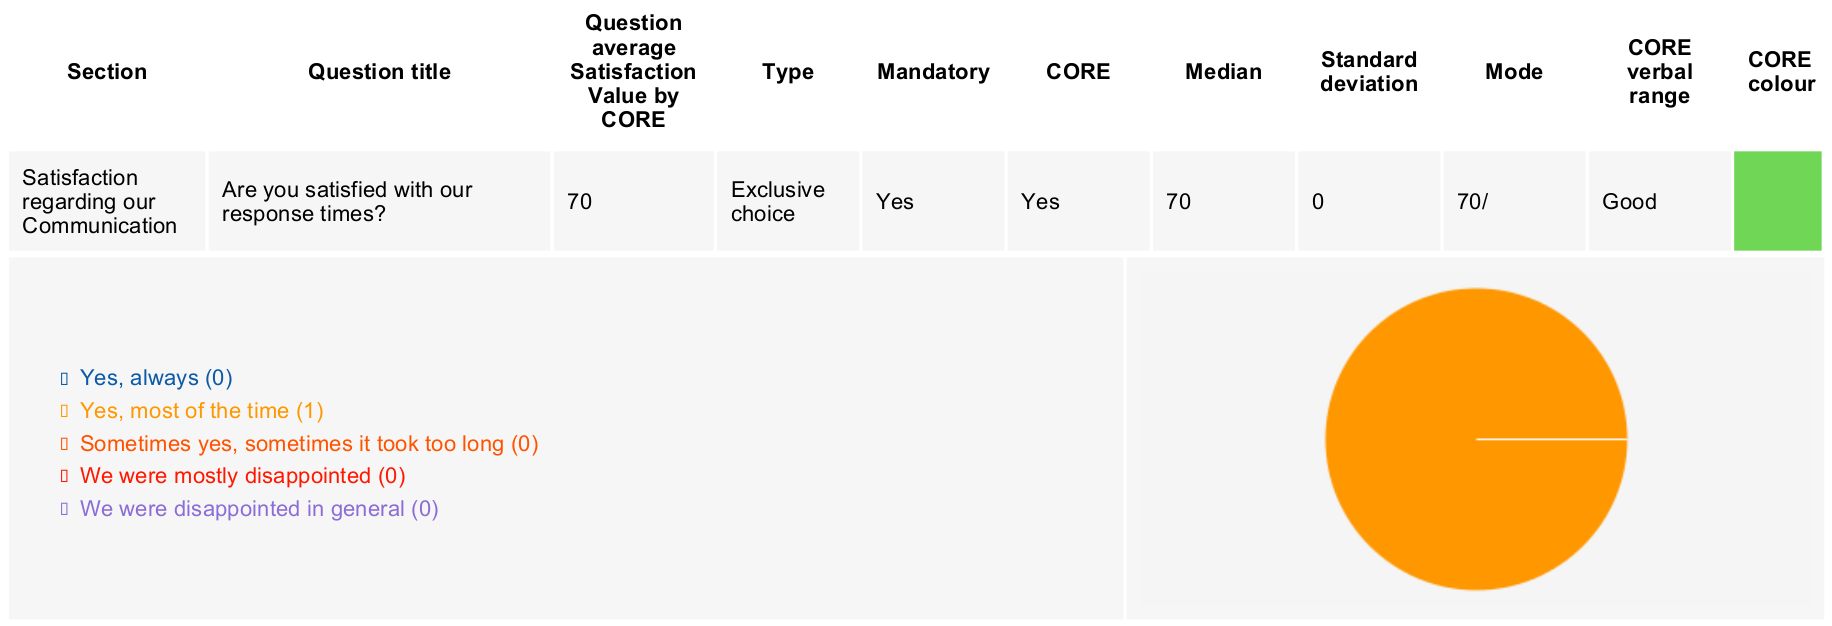
\includegraphics[width=\textwidth]{res/customerVoice/q3_results/q1.png}
%\caption{Overview of first Questionnaire's Results}
%\label{fig:resultsOverview}
\end{figure}

\begin{figure}
\centering
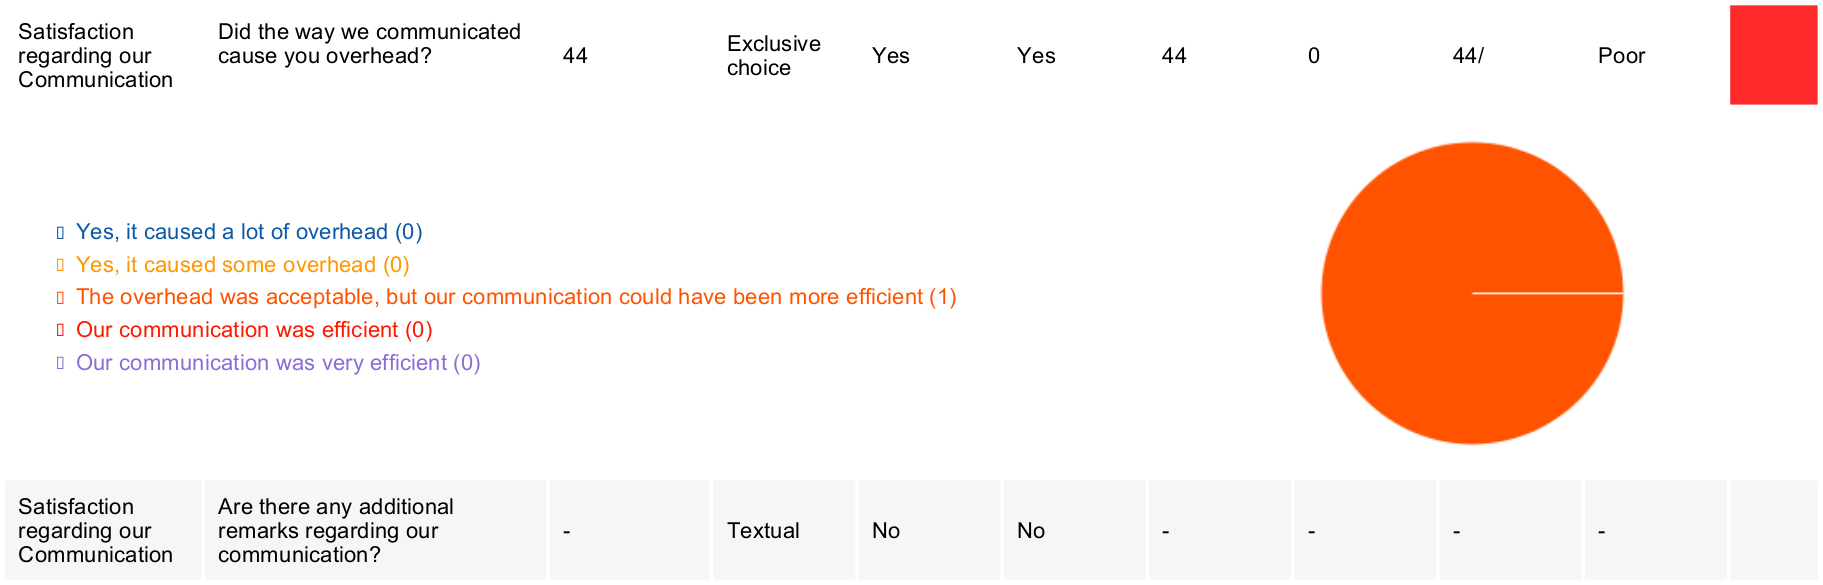
\includegraphics[width=\textwidth]{res/customerVoice/q3_results/q2.png}
%\caption{Overview of first Questionnaire's Results}
%\label{fig:resultsOverview}
\end{figure}

\begin{figure}
\centering
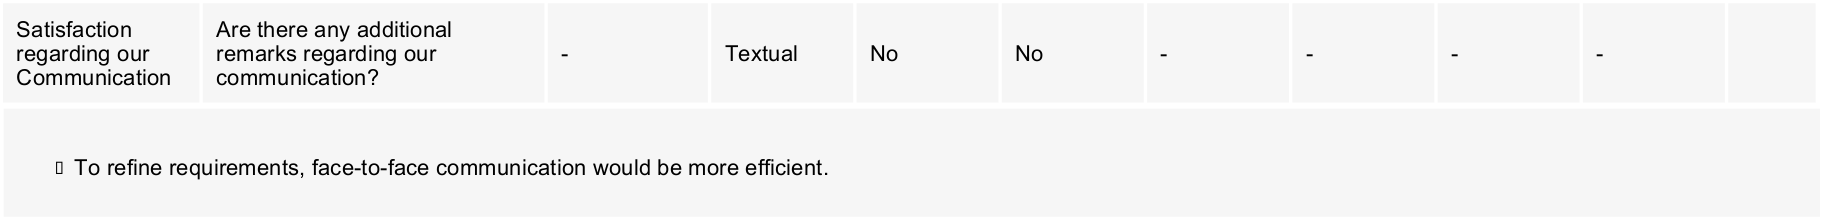
\includegraphics[width=\textwidth]{res/customerVoice/q3_results/q3.png}
%\caption{Overview of first Questionnaire's Results}
%\label{fig:resultsOverview}
\end{figure}

\begin{figure}
\centering
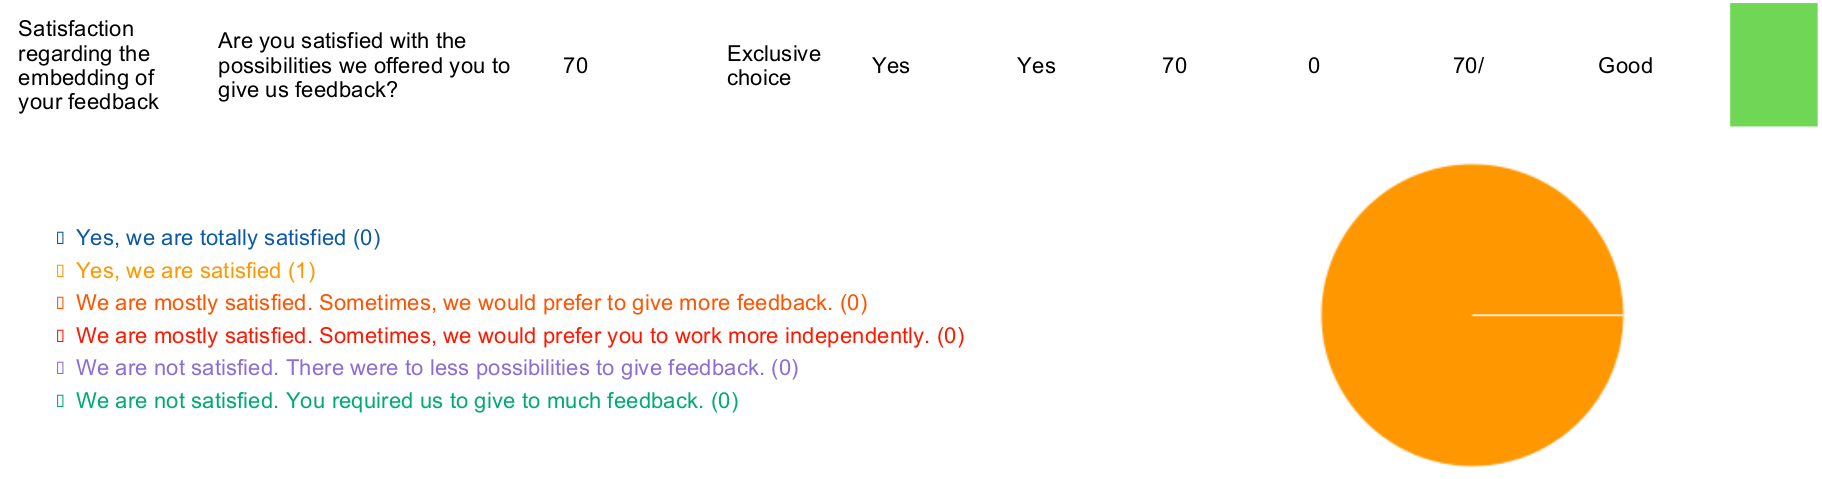
\includegraphics[width=\textwidth]{res/customerVoice/q3_results/q4.png}
%\caption{Overview of first Questionnaire's Results}
%\label{fig:resultsOverview}
\end{figure}

\begin{figure}
\centering
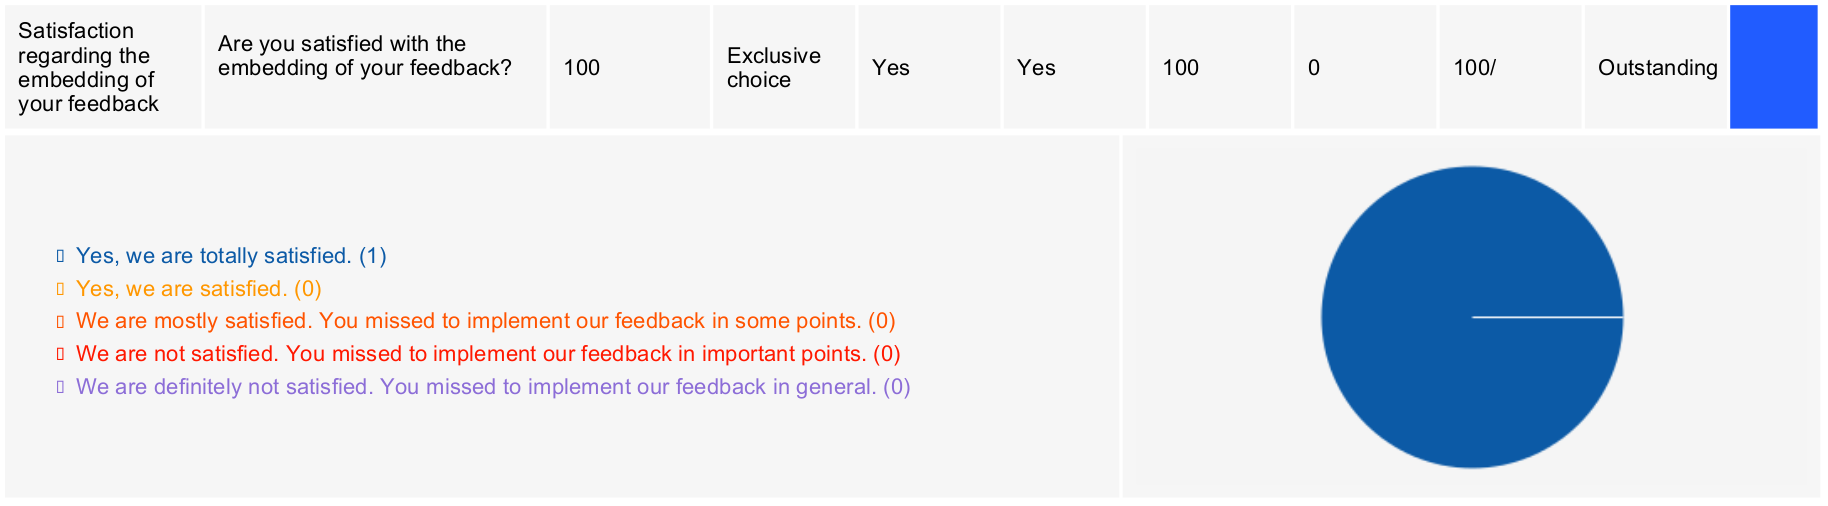
\includegraphics[width=\textwidth]{res/customerVoice/q3_results/q5.png}
%\caption{Overview of first Questionnaire's Results}
%\label{fig:resultsOverview}
\end{figure}

\begin{figure}
\centering
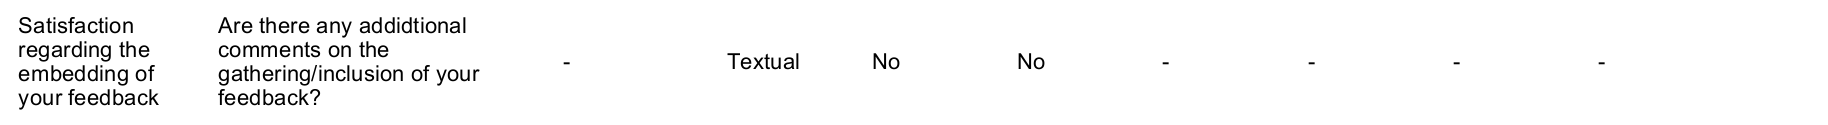
\includegraphics[width=\textwidth]{res/customerVoice/q3_results/q6.png}
%\caption{Overview of first Questionnaire's Results}
%\label{fig:resultsOverview}
\end{figure}

\begin{figure}
\centering
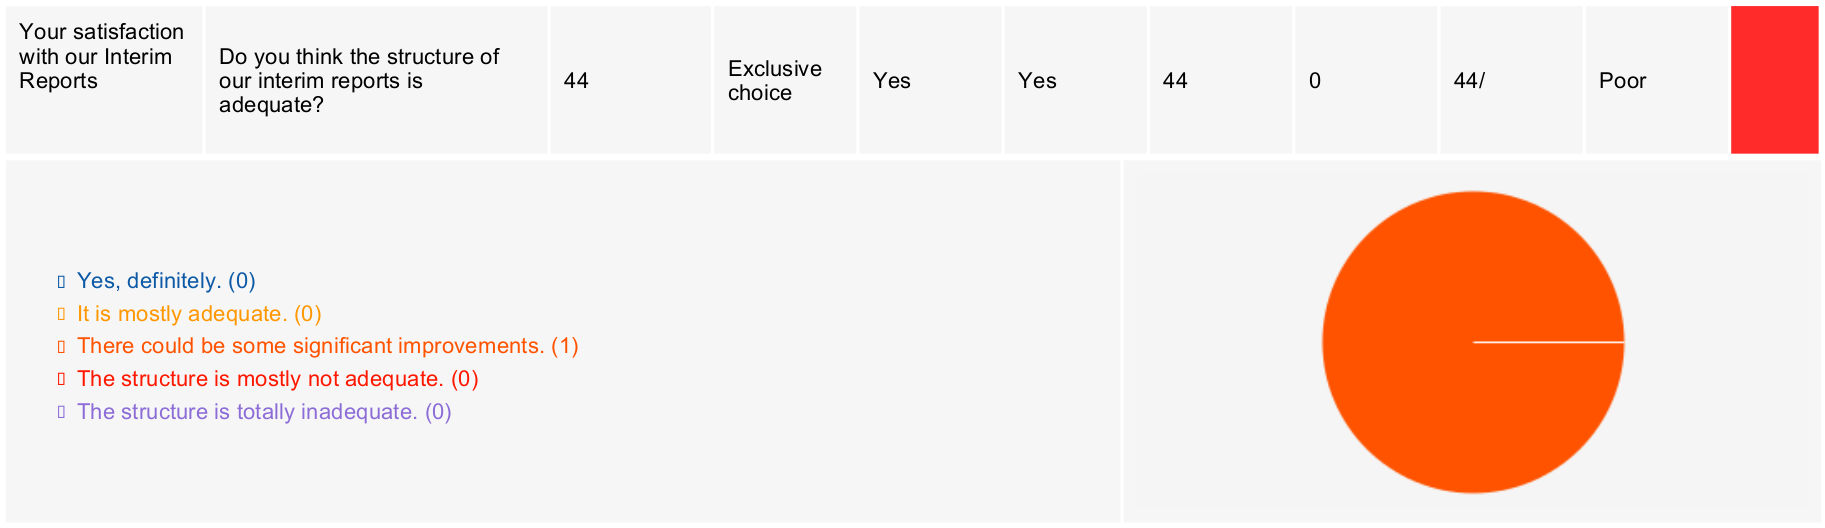
\includegraphics[width=\textwidth]{res/customerVoice/q3_results/q7.png}
%\caption{Overview of first Questionnaire's Results}
%\label{fig:resultsOverview}
\end{figure}

\begin{figure}
\centering
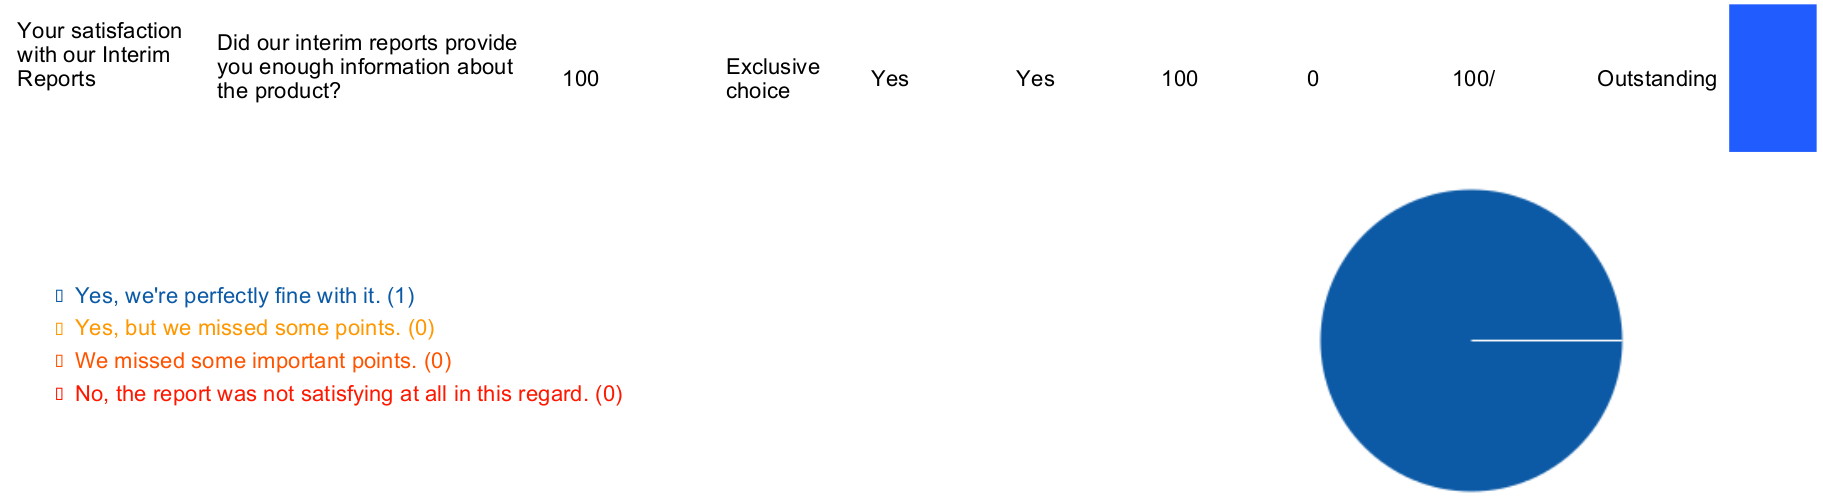
\includegraphics[width=\textwidth]{res/customerVoice/q3_results/q8.png}
%\caption{Overview of first Questionnaire's Results}
%\label{fig:resultsOverview}
\end{figure}

\begin{figure}
\centering
\includegraphics[width=\textwidth]{res/customerVoice/q3_results/q9.png}
%\caption{Overview of first Questionnaire's Results} 
%\label{fig:resultsOverview}
\end{figure}

\begin{figure}
\centering
\includegraphics[width=\textwidth]{res/customerVoice/q3_results/q10.png}
%\caption{Overview of first Questionnaire's Results}
%\label{fig:resultsOverview}
\end{figure}

\begin{figure}
\centering
\includegraphics[width=\textwidth]{res/customerVoice/q3_results/q11.png}
%\caption{Overview of first Questionnaire's Results}
%\label{fig:resultsOverview}
\end{figure}

\begin{figure}
\centering
\includegraphics[width=\textwidth]{res/customerVoice/q3_results/q12.png}
%\caption{Overview of first Questionnaire's Results}
%\label{fig:resultsOverview}
\end{figure}

\FloatBarrier

\subsection{Gained Knowledge}
\label{sect:q3_results}

The knowledge that could be extracted from the last questionnaire cannot be
applied to the current project. Nevertheless, the gained
knowledge is very important in regard to our company's aim of continuous
improvement and can be applied to subsequent projects.

One of the questionnaire's outcomes is that the interim reports should be
improved. The two-columns-layout implicates the problem of pictures being too
small. In some points, e.g. if the progress of the project is stated, textual
descriptions might be avoided by using expressive charts.

In addition, our company will cherish the idea of face-to-face communication
being the most efficient way of clarifying open questions. The overall result of
the last feedback form is depicted in figure \ref{fig:resultsOverview3}.


\begin{figure}[h!]
\centering
\captionsetup{justification=centering}
\includegraphics[width=\textwidth]{res/customerVoice/q3_results/overview.png}
\caption{Overview of second Questionnaire's Results}
\label{fig:resultsOverview3}
\end{figure}

\chapter{Product Development and Production Life Cycle Analysis}
\vspace{-1cm}
\epigraph{\textbf{Author: } Simon Schneider, Timo Acquistapace }

\vspace{-1cm}
TODO: There should be some blabla. 

\section{Use Case Diagram}

Based on the requirements that were agreed on with the customer, two main use
cases of the system can be found:

\begin{itemize}
\item{Drive out of a perpendicular Parking Lot}
\item{Drive out of a parallel Parking Lot}
\end{itemize}

Both use cases have in common that at the end of the successful process, the
user has to regain the control over its vehicle in a defined way. Additionally,
the user should always have the possibility to interrupt the process and regain
the control over the car, even if the process has not yet finished. Each of the
use cases are triggered by the driver as well as they are supported by various
sensors and control systems.

\begin{figure}
\centering
\captionsetup{justification=centering}
\includegraphics[width=\textwidth]{res/systemAnalysis/UseCase.png}
\caption{Overview of the System's Use Cases}
\label{fig:UseCases}
\end{figure}

\section{Sensor Overview}
To support the presented use cases, the system needs an overview of the cars
surrounding. Six sensors, two of them cameras and 4 of them distance sensors,
are placed in the car to provide this overview. The placement of the sensors can be
retrieved from figure \ref{fig:SensorOverview}.

The sensors that are placed in the middle of the car�s front and rear are
cameras. In many cases cameras are already integrated in the car and provide the
user a realistic image of its surrounding. The distance sensors at the corners
of the bumpers might be radar- or ultrasonic-sensors. Radar sensors have the
advantage, that they might be placed within the bumper and that they are
therefore not visible.

\begin{figure}
\centering
\captionsetup{justification=centering}
\includegraphics[width=0.75\textwidth]{res/systemAnalysis/SensorOverview.png}
\caption{Overview of the System' Sensors}
\label{fig:SensorOverview}
\end{figure}

\section{Context Diagram}

After the use cases and the required sensors have been found, the context of the
system to develop can be determined (see figure \ref{fig:ContextDiagram}).
Dataflows are depicted with solid arrows while signals that are used to control
the systems are sketched with dashed arrows.

Beside the sensor information, the graphical representation of the process and
the information that is sent to the car�s control systems, there exist two
systems that are used to interrupt the process of leaving a parking lot. If a
driver sits in the car and presses the break pedal, the process will be
interrupted immediately and the driver will regain the control over its vehicle.
If the whole process is controlled remotely without the driver sitting in its
car, the external application that controls the process should act as a dead
man�s switch that is operated by the user. If the signal from this application
is no more retrieved by the system, the process should be interrupted.


\begin{figure}
\centering
\captionsetup{justification=centering}
\includegraphics[width=\textwidth]{res/systemAnalysis/ContextDiagram.png}
\caption{Context Diagram of the System}
\label{fig:ContextDiagram}
\end{figure}

\section{Activity Diagrams}

Nachdem in den vorangegangen Kapiteln sowohl die Use cases als auch die
beteiligten Sensoren beschrieben wurden wird in diesem Kapitel der ablauf des
Perpendicular parking und des Parallel parking mithilfe von activity diagrammen
beschrieben. Ein activity diagram visualisiert die Dynamik und das Verhalten des
systems und tr�gt somit zu einem besseren Verst�ndnis des prozessablaufes bei. 

\subsection{Activity Diagram Reverse Perpendicular Parking}

Beim verlassen einer Perpendicular Parksituation gibt es verschiedene F�lle zu
betrachten die das System beinflussen k�nnen bzw daran hindern k�nnen gefahrlos
auszuparken. Ausserdem gibt es verschiedene Ausgangslagen, in welcher sich das
Fahrzeug befinden kann bevor der Ausparkvorgang gestartet wird. Zu diesem
Zweck wird im folgenden der Best- und der Worst Case der Ausgangslagen
beschrieben. Der Prozessablauf kann Figure \ref{fig:ActivityPerpendicular}
entnommen werden.

\begin{itemize}
\item \textbf{Best Case} \newline
Beim Best Case handelt es sich um eine Ausgangslage, bei welcher sich kein
Obstacle auf der fahrerseite des Fahrzeuges befindet. Dies wird mithilfe der
Sensoren des Fahrzeuges ermittelt. Der Gruund hierf�r ist es, dass beim
r�ckw�rtigen Ausparken das Fahrzeug direkt einlenken und zur�cksetzen kann.
Dabei ist es f�r den Reverse Perpendicular Parking Vorgang nicht von Bedeutung
ob sich ein Obstacle auf der Beifahrer seite befindent, da dies den
Ausparkvorgang nicht beeintr�chtigt. Es wird nun solange zur�ckgesetzt, bis das
Fahrzeug die Fahrbahn mithilfe der Kamera erkennt. Ausserdem wird zus�tzlich
gepr�ft, ob sich ein Fahrzeug, Fahrrad oder eine Person auf der Fahrbahn befindet. Falls dies der
Fall ist stoppt das Fahrzeug und wartet bis das Hinderniss beseitigt ist.
Befindet sich kein Hinderniss auf der Fahrbahn kann der Ausparkvorgang
fortgesetzt und beendet werden.
\item \textbf{Worst Case} \newline
Beim Schlechtfall handelt es sich um eine Ausgangslage, bei welcher fahrerseitig
ein Obstacle befindet. Dadurch ver�ndert sich der Ablauf des Prozesses, denn es
kann nun nicht mehr sofort eingelenkt werden sondern es muss zuerst
zur�ckgesetzt werden. Hierbei wird auch wieder darauf geachtet, dass sich keine
Person, Fahrrad oder Fahrzeug auf der Fahrbahn befindet. Es wird solange
zur�ckgesetzt bis fahrereseitig kein Hinderniss mehr von den Sensoren erkannt
wird. Anschlie�end kann das Fahrzeug wieder einlenken und der darauf folgende
Ablauf ist identisch, wie der beim Best Case.
\end{itemize}

\begin{figure}
\centering
\captionsetup{justification=centering}
\includegraphics[width=\textwidth]{res/systemAnalysis/ActivityObstacleTransversal.png}
\caption{Algorithm for leaving a perpendicular Parking Situation}
\label{fig:ActivityPerpendicular}
\end{figure}

\subsection{Activity Diagram Parallel Parking}

Auch beim verlassen einer Parallel Parksituation gibt es wiederum verschiedene
Ausgangslagen zu betrachten, die das System beinflussen k�nnen bzw daran hindern
k�nnen gefahrlos auszuparken. Analoge zum Reverse Perpendicular Parking wird im
folgenden der Best- und der Worst Case der Ausgangslagen beschrieben. 
Der Prozessablauf kann Figure \ref{fig:ActivityParallel} entnommen werden.

\begin{itemize}
\item \textbf{Best Case} \newline
In diesem Szenario ist der Best Case der, in welchem sich kein Hinderniss vor
dem Fahrzeug befindet. Dadurch kann das Fahrzeug direkt so einlenken, dass die
Reifen weg vom Bordstein zeigen und anschlie�end Vorw�rtsfahren. Beim
Vorw�rtsfahren wird weiterhin gepr�ft, ob sich kein Hinderniss vor dem Fahrzeug
befindet. Es wird nun solange Vorw�rts gefahren, bis die Kamera die Fahrbahn
erkennt. Ausserdem wird gepr�ft, dass sich keine Hindernisse auf der Fahrbahn
befinden. Ist dies der Fall so wird der Ausparkvorgang beendet. Andernfalls
stoppt das Fahrzeug und setzt erst mit dem Ausparkvorgang fort, sobald das
Hinderniss weg ist.
\item \textbf{Worst Case} \newline
Im Schlechtfall befindet sich sowohl vor dem Fahrzeug als auch hinter dem
Fahrzeug jeweils ein Obstacle. Dies bedeutet das Fahrzeug setzt soweit zur�ck
bis es einen minimalen Abstand zum Hinderniss hat. Anschlie�end dreht es die
R�der vom Bordstein weg und f�hrt vorw�rts. Erkennt das Fahrzeug nun ein
Hinderniss vor sich, so h�lt es an, dreht seine R�der zum Bordstein hin und
f�hrt r�ckw�rts. Dies tut es wiederum solange bis es kurz vor dem r�ckw�rtigen
Hinderniss steht. Anschlie�end werden die R�der wieder vom Bordstein weggedreht
und solange vorw�rts gefahren bis die Stra�e erkennt wird. Der folgende Ablauf
des Ausparkprozesses ist wiederum identisch zum Best Case.
\end{itemize}

\begin{figure}
\centering
\captionsetup{justification=centering}
\includegraphics[width=\textwidth]{res/systemAnalysis/ActivityObstacleLenghtwise.png}
\caption{Algorithm for leaving a parallel Parking Situation}
\label{fig:ActivityParallel}
\end{figure}

\section{Design Sketches}

A first design sketch has been developed (see figure \ref{fig:initialMockup})
and the customer�s feedback on the design has been gathered, this feedback is
used to create refined mockups. Since the customer requests two designs -- one
for the day and one for the night-mode -- two of these refined designs are
developed.

These newly designed mockups also take the customer�s feedback into account that
some outputs should be simplified and that the area where the sensor information
is presented should not be reduced. Instead, the area presenting the aerial view
is reduced and the sensor information are presented in a wider area.

\begin{figure}
\centering
\captionsetup{justification=centering}
\includegraphics[width=0.75\textwidth]{res/systemAnalysis/darkskin.png}
\caption{Dark Skin of the final Design Sketch}
\label{fig:darkskin}
\end{figure}

\begin{figure}
\centering
\captionsetup{justification=centering}
\includegraphics[width=0.75\textwidth]{res/systemAnalysis/brightskin.png}
\caption{Bright Skin of the final Design Sketch}
\label{fig:brightskin}
\end{figure}
 

\chapter{Facilitation and Monitoring of the Process}
\vspace{-1cm}
\epigraph{\textbf{Author: } Hans \newline \textbf{Contributor(s): }Wurst}

\chapter{Conclusions}
\vspace{-1cm}
\epigraph{\textbf{Author: } Markus Just, Timo Acquistapace, Simon Schneider,
Wojciech Lesnianski}

\section{Conclusion - Markus Just}

\section{Conclusion - Timo Acquistapace}
This project was the first one in my educational experience that included a
detailed process of project management. As a consequence, it was on the one hand
very interesting to get an insight into the steps that could help to run a
project successfully. On the other hand, there are some points that would be
done in a different way the next time a similar project is set up, e.g. the
assignment of roles. The roles were initially assigned to the team members with
regard to their technical skills and knowledge.  Since every team member was
also assigned to do some work in the area of project management, there occurred
some interdependencies that were not considered in the assignment of roles. An
exemplary interdependence in the current project is the following: To evaluate
the customer's satisfaction with the first drafts of the system, it is very
helpful if a design sketch is available. However, the designer was not entrusted
with the task of evaluating the customer's satisfaction. To avoid additional
overhead for synchronization and waiting times, the initial assignment of roles
was defined down and the creation of mockups as well as their enhancement
according to the customer's feedback was assigned to the person that was
responsible for the involvement of the customer.

Embedding the customer's voice itself is proved itself expensive. After having
collected some experience with agile methods and their regular, but non-formal
events to collect feedback on a product or process, the way of using
questionnaires to determine the customer's satisfaction appears nonelastic and
complicated at the first glance. But over the course of the project, the
advantages of documented feedback became clear. The used tool to create the
questionnaires -- Satistica -- proved itself very helpful. Gathered feedback is
diagrammed clearly by Satistica and single questions as well as whole sections
of questions can be evaluated easily regarding the point if the answers fit the
expectations. It is therefore very easy to determine the areas of work where
some improvements have to take place. Nevertheless, written feedback that does
not offer the possibility to make a query directly could also be misunderstood
like every written document. It has to be kept in mind that creating good
questionnaires is a part of social science and there are many points to
consider. Concluding, I would value direct discussions over feedback
questionnaires. If this is not possible, Satistica anyway offers good support in
collecting a customer's feedback.

The market analysis conducted exhibits the greatest deviation from the way it
would be done in a commercial project. Whilst the prices of needed hardware
parts are only gathered by a research on the internet, contacting the different
manufacturer would be inevitable in a commercial project. The manufacturers may
provide more favourable conditions if a larger amount of pieces is ordered and
they may also counsel our company on the selection of the products. If the
analysis is done in a very early stage, even before the project team is chosen,
the persons that already published research projects like Katsev and Braun might
be contacted and asked to contribute to the project by bringing in their
experience. The greatest weakness of the conducted market analysis is the way
how the competitors' products were analysed. While the information was again
gathered by research on the internet, a commercial project would require to test
the products that are already available on the market. Only this it is possible
to get an impression of how these product might be improved and how the
competitors could thereby be overcome.

\section{Conclusion - Simon Schneider}

\section{Conclusion - Wojciech Lesnianski} 

\listoftables
\listoffigures
\bibliography{resources} 

\end{document}
